% Options for packages loaded elsewhere
\PassOptionsToPackage{unicode}{hyperref}
\PassOptionsToPackage{hyphens}{url}
\PassOptionsToPackage{dvipsnames,svgnames,x11names}{xcolor}
%
\documentclass[
  12pt,
]{article}
\usepackage{amsmath,amssymb}
\usepackage{lmodern}
\usepackage{iftex}
\ifPDFTeX
  \usepackage[T1]{fontenc}
  \usepackage[utf8]{inputenc}
  \usepackage{textcomp} % provide euro and other symbols
\else % if luatex or xetex
  \usepackage{unicode-math}
  \defaultfontfeatures{Scale=MatchLowercase}
  \defaultfontfeatures[\rmfamily]{Ligatures=TeX,Scale=1}
\fi
% Use upquote if available, for straight quotes in verbatim environments
\IfFileExists{upquote.sty}{\usepackage{upquote}}{}
\IfFileExists{microtype.sty}{% use microtype if available
  \usepackage[]{microtype}
  \UseMicrotypeSet[protrusion]{basicmath} % disable protrusion for tt fonts
}{}
\makeatletter
\@ifundefined{KOMAClassName}{% if non-KOMA class
  \IfFileExists{parskip.sty}{%
    \usepackage{parskip}
  }{% else
    \setlength{\parindent}{0pt}
    \setlength{\parskip}{6pt plus 2pt minus 1pt}}
}{% if KOMA class
  \KOMAoptions{parskip=half}}
\makeatother
\usepackage{xcolor}
\usepackage[margin=1in]{geometry}
\usepackage{longtable,booktabs,array}
\usepackage{calc} % for calculating minipage widths
% Correct order of tables after \paragraph or \subparagraph
\usepackage{etoolbox}
\makeatletter
\patchcmd\longtable{\par}{\if@noskipsec\mbox{}\fi\par}{}{}
\makeatother
% Allow footnotes in longtable head/foot
\IfFileExists{footnotehyper.sty}{\usepackage{footnotehyper}}{\usepackage{footnote}}
\makesavenoteenv{longtable}
\usepackage{graphicx}
\makeatletter
\def\maxwidth{\ifdim\Gin@nat@width>\linewidth\linewidth\else\Gin@nat@width\fi}
\def\maxheight{\ifdim\Gin@nat@height>\textheight\textheight\else\Gin@nat@height\fi}
\makeatother
% Scale images if necessary, so that they will not overflow the page
% margins by default, and it is still possible to overwrite the defaults
% using explicit options in \includegraphics[width, height, ...]{}
\setkeys{Gin}{width=\maxwidth,height=\maxheight,keepaspectratio}
% Set default figure placement to htbp
\makeatletter
\def\fps@figure{htbp}
\makeatother
\setlength{\emergencystretch}{3em} % prevent overfull lines
\providecommand{\tightlist}{%
  \setlength{\itemsep}{0pt}\setlength{\parskip}{0pt}}
\setcounter{secnumdepth}{5}
\newlength{\cslhangindent}
\setlength{\cslhangindent}{1.5em}
\newlength{\csllabelwidth}
\setlength{\csllabelwidth}{3em}
\newlength{\cslentryspacingunit} % times entry-spacing
\setlength{\cslentryspacingunit}{\parskip}
\newenvironment{CSLReferences}[2] % #1 hanging-ident, #2 entry spacing
 {% don't indent paragraphs
  \setlength{\parindent}{0pt}
  % turn on hanging indent if param 1 is 1
  \ifodd #1
  \let\oldpar\par
  \def\par{\hangindent=\cslhangindent\oldpar}
  \fi
  % set entry spacing
  \setlength{\parskip}{#2\cslentryspacingunit}
 }%
 {}
\usepackage{calc}
\newcommand{\CSLBlock}[1]{#1\hfill\break}
\newcommand{\CSLLeftMargin}[1]{\parbox[t]{\csllabelwidth}{#1}}
\newcommand{\CSLRightInline}[1]{\parbox[t]{\linewidth - \csllabelwidth}{#1}\break}
\newcommand{\CSLIndent}[1]{\hspace{\cslhangindent}#1}
\usepackage{setspace} \setstretch{1.15} \usepackage{float} \floatplacement{figure}{t}
\ifLuaTeX
  \usepackage{selnolig}  % disable illegal ligatures
\fi
\IfFileExists{bookmark.sty}{\usepackage{bookmark}}{\usepackage{hyperref}}
\IfFileExists{xurl.sty}{\usepackage{xurl}}{} % add URL line breaks if available
\urlstyle{same} % disable monospaced font for URLs
\hypersetup{
  colorlinks=true,
  linkcolor={cyan},
  filecolor={Maroon},
  citecolor={Blue},
  urlcolor={cyan},
  pdfcreator={LaTeX via pandoc}}

\title{~\Large Increased sexual dimorphism evolves in a fossil
stickleback following ecological release from fish piscivores}
\author{\large Allison Ozark\(^{1,*}\), Matthew Stuart\(^{2,3,*}\),
Raheyma Siddiqui\(^1\), Akhil Ghosh\(^{2,3}\)\\
\large Samantha Swank\(^1\), Michael A. Bell\(^4\), Gregory J.
Matthews\(^{2,3}\), and Yoel E. Stuart\(^{1,+}\)\\
\vspace{-1.1mm}\\
\large \(^1\) Department of Biology, Loyola University Chicago, Chicago,
IL, USA \vspace{-1.1mm}\\
\large \(^2\) Department of Mathematics and Statistics, Loyola
University Chicago, Chicago, IL, USA \vspace{-1.1mm}\\
\large \(^3\) Center for Data Science and Consulting, Loyola University
Chicago, Chicago, IL, USA \vspace{-1.1mm}\\
\large \(^4\) University of California Museum of Paleontology, Berkeley,
CA, USA \vspace{-1.1mm}\\
\large \(^*\) Equal contribution \vspace{-1.1mm}\\
\large \(^+\) Corresponding:
\href{mailto:ystuart@luc.edu}{\nolinkurl{ystuart@luc.edu}}
\vspace{-1.1mm}}
\date{}

\begin{document}
\maketitle
\begin{abstract}
Everyone loves the stickle \vspace{2mm}\\
\emph{Keywords}: Stickle
\end{abstract}

\newcommand{\iid}{\overset{iid}{\sim}}

\newpage

\hypertarget{sec:intro}{%
\section{Introduction}\label{sec:intro}}

Ecological release theory suggests that a population's niche should
change when important species interactions (e.g., resource competition)
are relaxed or removed (reviewed in Herrmann, Stroud, and Losos
(\protect\hyperlink{ref-Herrmannetal2021}{2021})). Removal is posited to
create ecological opportunities---i.e., aspects of the niche become
newly accessible, and the focal population shifts and/or expands its
resource use to the new opportunity (Parent and Crespi
(\protect\hyperlink{ref-ParentandCrespi2009}{2009}); Herrmann, Stroud,
and Losos (\protect\hyperlink{ref-Herrmannetal2021}{2021})). Ecological
release may then be followed by adaptive morphological evolution (Parent
and Crespi (\protect\hyperlink{ref-ParentandCrespi2009}{2009});
Herrmann, Stroud, and Losos
(\protect\hyperlink{ref-Herrmannetal2021}{2021})). For example, a
population undergoing ecological release can experience disruptive
selection on males and females stemming from intraspecific competition
over newly accessible resources (Bolnick and Doebeli
(\protect\hyperlink{ref-BolnickandDoebeli2003}{2003}); Bolnick and Lau
(\protect\hyperlink{ref-BolnickandLau2008}{2008}); Cooper, Gilman, and
Boughman (\protect\hyperlink{ref-Cooperetal2011}{2011})). This is
predicted to result in intersexual divergence in habitat use and
associated phenotypes (Schoener
(\protect\hyperlink{ref-Schoener1968}{1968}); Shine
(\protect\hyperlink{ref-Shine1989}{1989}); Bolnick and Doebeli
(\protect\hyperlink{ref-BolnickandDoebeli2003}{2003}); Butler and Losos
(\protect\hyperlink{ref-Butleretal2007}{2007}); Bolnick and Lau
(\protect\hyperlink{ref-BolnickandLau2008}{2008}); Cooper, Gilman, and
Boughman (\protect\hyperlink{ref-Cooperetal2011}{2011}); but see Stuart
et al. (\protect\hyperlink{ref-Stuartetal2021}{2021}); Blain
(\protect\hyperlink{ref-Blain2022}{2022})). Such competition-driven
``intraspecific character displacement'' between the sexes is therefore
one explanation for the evolution of sexual dimorphism (Pfennig and
Pfennig (\protect\hyperlink{ref-PfennigandPfennig2012}{2012}); De Lisle
and Rowe (\protect\hyperlink{ref-DeLisleandRowe2015}{2015}); De Lisle
and Rowe (\protect\hyperlink{ref-DeLisleandRowe2017}{2017}), De Lisle,
Paiva, and Rowe (\protect\hyperlink{ref-DeLisleetal2018}{2018})).

Much of the theory and empirical data for character displacement between
the sexes is based on release from resource competition specifically
(e.g., Bolnick and Doebeli
(\protect\hyperlink{ref-BolnickandDoebeli2003}{2003}); Cooper, Gilman,
and Boughman (\protect\hyperlink{ref-Cooperetal2011}{2011}); Pfennig and
Pfennig (\protect\hyperlink{ref-PfennigandPfennig2012}{2012}); De Lisle
and Rowe (\protect\hyperlink{ref-DeLisleandRowe2015}{2015}); De Lisle,
Paiva, and Rowe (\protect\hyperlink{ref-DeLisleetal2018}{2018})).
However, release from predation should also result in ecological release
followed by the evolution of increased sexual dimorphism because the
absence of predators should generate ecological opportunity (Reimchen
and Nosil (\protect\hyperlink{ref-ReimchenandNosil2004}{2004}); Parent
and Crespi (\protect\hyperlink{ref-ParentandCrespi2009}{2009});
Herrmann, Stroud, and Losos
(\protect\hyperlink{ref-Herrmannetal2021}{2021})).

Here, we tested the prediction that a release from predation should
result in the evolution of increased sexual dimorphism using a
well-preserved, finely-resolved sequence of a fossil threespine
stickleback fish (Gasterosteus doryssus). The sequence in this
depositional environment is comprised of two lineages (Bell
(\protect\hyperlink{ref-Bell2009}{2009}); Cerasoni, Bell, and Stuart
(\protect\hyperlink{ref-Cerasonietal2024}{2024})). Lineage I was a
low-armor form with zero to one dorsal spines and highly reduced
pelvises, on average. It lasted for at least 93,000 years before it was
replaced suddenly by a second lineage (Bell, Baumgartner, and Oslon
(\protect\hyperlink{ref-Belletal1985}{1985})). Lineage II appeared in
the depositional environment fully armored, with complete pelvic
girdles, two pelvic spines, and three dorsal spines, on average (Bell,
Travis, and Blouw (\protect\hyperlink{ref-Belletal2006}{2006}); Stuart,
Travis, and Bell (\protect\hyperlink{ref-Stuartetal2020}{2020})). It
then immediately began evolving adaptive reduction in its armor traits
(Hunt, Bell, and Travis (\protect\hyperlink{ref-Huntetal2008}{2008});
Stuart, Travis, and Bell (\protect\hyperlink{ref-Stuartetal2020}{2020}))
until it reached the same low-armor state previously held by lineage I.
The observation of 93,000 years of low-armor stasis in lineage I (Bell,
Baumgartner, and Oslon (\protect\hyperlink{ref-Belletal1985}{1985})) and
the observation of rapid evolution of armor loss by lineage II, both
suggest that this depositional environment lacked piscivorous fish
(e.g., trout and other salmonids known to prey on modern threespine
stickleback). Armor maintenance in extant threespine stickleback
(Gasterosteus aculeatus) correlates strongly the presence of vertebrate
piscivores; populations with less predation pressure typically have less
armor (Reimchen (\protect\hyperlink{ref-Reimchen1994}{1994}), Reimchen
and Nosil (\protect\hyperlink{ref-ReimchenandNosil2004}{2004}); Bell et
al. (\protect\hyperlink{ref-Belletal1993}{1993}); Roesti et al.
(\protect\hyperlink{ref-Roestietal2023}{2023})). Consistently, only
three fossil trout have been recorded from this paleolake basin, sampled
from the same rock that has revealed \textgreater15,000 threespine
stickleback fossils as well as occasional killifish (Fundulus
nevadensis) (Bell (\protect\hyperlink{ref-Bell2009}{2009}); Cerasoni,
Bell, and Stuart (\protect\hyperlink{ref-Cerasonietal2024}{2024})).
Finally, tooth wear data from the lineage II sequence suggest that
individuals in this lineage began eating more planktonic prey over time,
expanding toward an open-water niche from the benthic, bottom-feeding
niche they started with (Purnell et al.~2007). That this expansion into
open water by lineage II coincided with armor reduction is further
indicative of a limnetic system with fewer salmonid piscivores (Schluter
and McPhail (\protect\hyperlink{ref-SchluterandMcPhail1992}{1992});
Vamosi and Schluter
(\protect\hyperlink{ref-VamosiandSchluter2004}{2004}); Roesti et al.
(\protect\hyperlink{ref-Roestietal2023}{2023})). In sum, we infer that
lineage II likely started in a nearby paleolake basin that had predators
since it was armored when it arrived (Bell
(\protect\hyperlink{ref-Bell2009}{2009}); Cerasoni, Bell, and Stuart
(\protect\hyperlink{ref-Cerasonietal2024}{2024})). Lineage II then
experienced release from predators and dietary expansion in the focal
paleolake basin, generating a scenario consistent with the starting
conditions for models predicting the evolution of increased sexual
dimorphism following ecological release.

A major challenge in the study of fossilized sexual dimorphism is
assigning sex to individual specimens in the first place (Hone and
Mallon (\protect\hyperlink{ref-HoneandMallon2017}{2017}); Mallon
(\protect\hyperlink{ref-Mallon2017}{2017}); Saitta et al.
(\protect\hyperlink{ref-Saittaetal2020}{2020})). This typically cannot
be done directly, except for taxa whose sexes are distinguished by the
presence or absence of sex-specific characters that preserve well.
Instead, paleobiologists often resort to statistical detection of sex
and sexual dimorphism, including tests for normality and bimodality in
trait distributions (e.g., Mallon
(\protect\hyperlink{ref-Mallon2017}{2017})), mixture modeling (e.g.,
Mallon (\protect\hyperlink{ref-Mallon2017}{2017})), divergence in growth
curves (e.g., Saitta et al.
(\protect\hyperlink{ref-Saittaetal2020}{2020})), and emphasis on effect
size statistics rather than significance testing (e.g., Saitta et al.
(\protect\hyperlink{ref-Saittaetal2020}{2020})). However, dimorphic
signal can be masked by noise introduced by factors both biological and
artifactual, including extended growth during ontogeny, age-based bias
in survivorship, small sample sizes, time averaging, and taphonomic bias
(Godfrey, Lyon, and Sutherland
(\protect\hyperlink{ref-Godfreyetal1993}{1993}); Koscinski and
Pietraszewski
(\protect\hyperlink{ref-KoscinskiandPietraszewski2004}{2004}); Hone and
Mallon (\protect\hyperlink{ref-HoneandMallon2017}{2017}); reviewed in
Mallon (\protect\hyperlink{ref-Mallon2017}{2017}); reviewed in Saitta et
al. (\protect\hyperlink{ref-Saittaetal2020}{2020})). Thus, the best
approach to sex classification is likely one of total evidence (Saitta
et al. (\protect\hyperlink{ref-Saittaetal2020}{2020})), including
comparison to closely-related, extant species of known sex (e.g., Hone
and Mallon (\protect\hyperlink{ref-HoneandMallon2017}{2017}); Saitta et
al. (\protect\hyperlink{ref-Saittaetal2020}{2020})).

For our study, we inferred sex in G. doryssus fossils by comparing
multivariate morphological trait data from lineage II samples to the
same multivariate trait set collected from multiple populations in the
closely-related, extant Threespine Stickleback species complex
(Gasterosteus aculeatus). Crucially, we determined G. aculeatus sex
directly via dissection and/or PCR genotyping. This enabled us to use
Multiple Imputation by Chained Equations (MICE; Buuren and
Groothuis-Oudshoorn (\protect\hyperlink{ref-MICE}{2011})) to build a
predictive multiple imputation algorithm (Little and Rubin
(\protect\hyperlink{ref-little2002statistical}{2002})) based on the
multivariate morphology of G. aculeatus individuals of known sex. We
applied this algorithm to the fossil data to impute individual sex based
on morphology, treating fossil sex as a missing variable. With sex
assigned to fossil specimens (and accounting for uncertainty in those
assignments), we fit a modified Ornstein-Uhlenbeck (OU) (Uhlenbeck and
Ornstein (\protect\hyperlink{ref-OUProcess}{1930})) model using a
Bayesian framework to test for evolution of sexual dimorphism in each
trait over \textasciitilde16,000 years of lineage II. We hypothesized
that sexual dimorphism should increase following ecological release from
predators.

\hypertarget{sec:data}{%
\section{Data}\label{sec:data}}

\hypertarget{fossil-specimen-data}{%
\subsection{Fossil Specimen Data}\label{fossil-specimen-data}}

We used Gasterosteus doryssus data that were previously reported by
Stuart, Travis, and Bell (\protect\hyperlink{ref-Stuartetal2020}{2020}),
Voje, Bell, and Stuart (\protect\hyperlink{ref-Vojeetal2022}{2022}), and
Siddiqui et al. (\protect\hyperlink{ref-Siddiquietal2024}{2024}).
Briefly, the data were collected from fossil Series K from Quarry D
(Cerasoni, Bell, and Stuart
(\protect\hyperlink{ref-Cerasonietal2024}{2024})), dug from an open pit
diatomite mine at 9.526° N, 119.094° W, near Fernley, Nevada, USA.
Series K consisted of 18 samples taken at \textasciitilde1000-year
intervals, and mean sample times span \textasciitilde16,363 years. Fish
from series K were measured for 16 ecomorphological traits related to
armor, swimming, and feeding (Table 1). Series K started at a previously
documented horizon when a low armored lineage of stickleback with zero
to one dorsal spines, zero pelvic spines, and highly reduced pelvises
(i.e., lineage I described above) was completely replaced by a high
armored lineage of stickleback with three dorsal spines, two pelvic
spines, and complete pelvises (i.e., lineage II described above) (Bell,
Travis, and Blouw (\protect\hyperlink{ref-Belletal2006}{2006}); Bell
(\protect\hyperlink{ref-Bell2009}{2009}); Stuart, Travis, and Bell
(\protect\hyperlink{ref-Stuartetal2020}{2020})). Lineage II subsequently
evolved reduction in armor, body size, and traits related to swimming
and feeding (Bell, Travis, and Blouw
(\protect\hyperlink{ref-Belletal2006}{2006}); Stuart, Travis, and Bell
(\protect\hyperlink{ref-Stuartetal2020}{2020}); Siddiqui et al.
(\protect\hyperlink{ref-Siddiquietal2024}{2024})). The tempo and mode of
armor reduction during this sequence suggests adaptive evolution by
natural selection (Hunt, Bell, and Travis
(\protect\hyperlink{ref-Huntetal2008}{2008})), and we focus on the
multivariate evolution of sexual dimorphism by this second lineage.

The lineage II fossil data consist of 814 specimens of unknown sex
sampled across 18 time periods spaced \textasciitilde1000 years apart.
Figure 1 shows the sample size for each of the 18 samples. There are at
least 22 specimens in each sample with a high of 67 specimens in sample
7.

\begin{figure}

{\centering 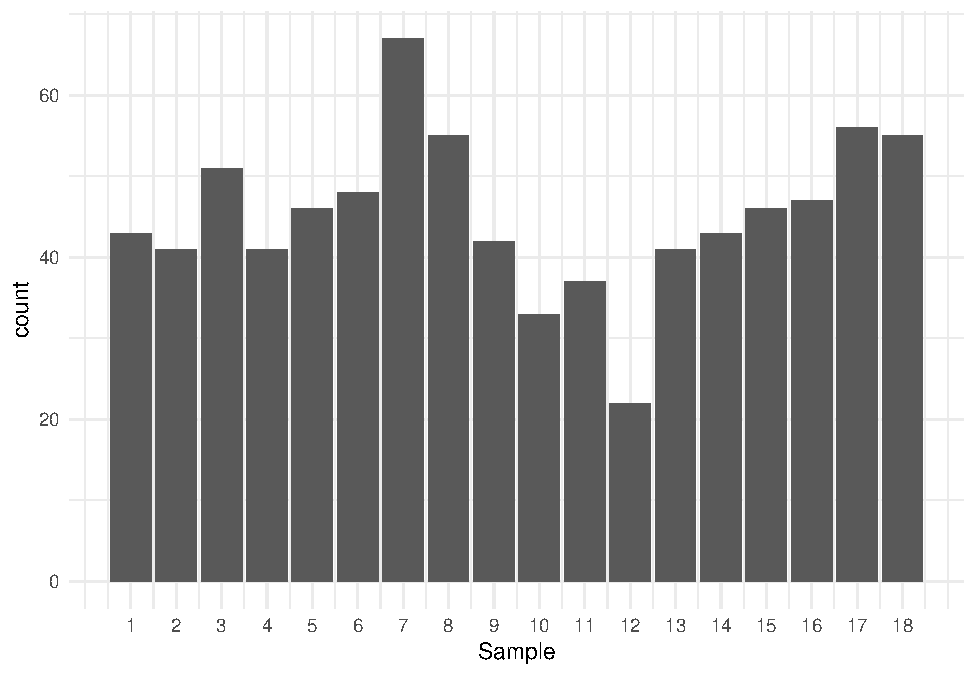
\includegraphics{paper_files/figure-latex/unnamed-chunk-2-1} 

}

\caption{Fossil sample size for each time period}\label{fig:unnamed-chunk-2}
\end{figure}

\begin{longtable}[]{@{}
  >{\raggedright\arraybackslash}p{(\columnwidth - 4\tabcolsep) * \real{0.3492}}
  >{\raggedright\arraybackslash}p{(\columnwidth - 4\tabcolsep) * \real{0.1905}}
  >{\raggedright\arraybackslash}p{(\columnwidth - 4\tabcolsep) * \real{0.4603}}@{}}
\caption{Traits and trait descriptions. `sc' denotes size correction of
trait against standard length. Names of bones follow Bowne
(\protect\hyperlink{ref-Bowne1994}{1994}) unless otherwise
noted.}\tabularnewline
\toprule()
\begin{minipage}[b]{\linewidth}\raggedright
Trait Name
\end{minipage} & \begin{minipage}[b]{\linewidth}\raggedright
Trait Code
\end{minipage} & \begin{minipage}[b]{\linewidth}\raggedright
Trait Description
\end{minipage} \\
\midrule()
\endfirsthead
\toprule()
\begin{minipage}[b]{\linewidth}\raggedright
Trait Name
\end{minipage} & \begin{minipage}[b]{\linewidth}\raggedright
Trait Code
\end{minipage} & \begin{minipage}[b]{\linewidth}\raggedright
Trait Description
\end{minipage} \\
\midrule()
\endhead
Standard Length & \texttt{stl} & Distance from anterior tip of
premaxilla to posterior end of last vertebra (hypural plate) \\
Dorsal Spine & \texttt{mds} & Number of dorsal spines from 0 to 3 \\
Dorsal Fin Ray & \texttt{mdf} & Number of bones in the dorsal fin
posterior to the third dorsal spine (i.e., soft dorsal fin rays) \\
Anal Fin Ray & \texttt{maf} & Number of bones in the anal fin posterior
to the anal spine (i.e., soft dorsal fin rays) \\
Abdominal Vertebra & mav & Number of vertebrae anterior to the first
vertebra contacting an anal fin pterygiophore (Aguirre et al.~2014) \\
Caudal Vertebra & \texttt{mcv} & Number of vertebrae posterior to and
including the first vertebra contacting an anal fin pterygiophore
(Aguirre et al.~2014) \\
Pterygiophore number & \texttt{mpt} & Number of pterygiophores anterior
to but excluding the pterygiophore under the third dorsal spine, which
is immediately anterior to and contiguous with the dorsal fin \\
Pelvic Spine length & \texttt{lps.sc} & Length from the base of one
pelvic spine above its articulation with the pelvic girdle to its distal
tip \\
Ectocoracoid & \texttt{ect.sc} & Length between the anterior and
posterior tips of the shoulder girdle base (i.e., ectocoracoid) \\
Pelvic Girdle & \texttt{tpg.sc} & Length between the anterior to
posterior tips along midline. If vestigial, the sum of longest
anterior-posterior axis for the vestiges \\
Cleithrum length & \texttt{cle.sc} & Length from free dorsal tip to
ventral tip of the cleithrum on the anterior margin of the shoulder
girdle (i.e., cleithrum) \\
Premaxilla & \texttt{pmx.sc} & Length from the anterior tip of the
premaxilla to the distal tip of the ascending process of the
premaxilla \\
Dorsal Spine & \texttt{Ds\#.sc\#\ =\ 1,2,or\ 3} & Length from the base
of a dorsal spine above the pterygiophore to its distal tip along the
anterior edge \\
Pterygiophore & \texttt{lpt.sc} & Distance between the anterior to
posterior tips of the pterygiophore immediately preceding the 3rd dorsal
spine (when present) \\
\bottomrule()
\end{longtable}

\hypertarget{extant-specimen-data}{%
\subsection{Extant Specimen data}\label{extant-specimen-data}}

To span the gamut of stickleback diversity for our predictive imputation
model, we sampled modern stickleback from lakes containing generalist
stickleback populations (Hendry et al.
(\protect\hyperlink{ref-Hendryetal2009}{2009}); Bolnick
(\protect\hyperlink{ref-Bolnick2011}{2011})) and from lakes containing
benthic-limnetic species pairs (Baumgartner, Bell, and Weinberg
(\protect\hyperlink{ref-Baumgartneretal1988}{1988}); Schluter and
McPhail (\protect\hyperlink{ref-SchluterandMcPhail1992}{1992})). The
generalist populations used here were the remainder of collections made
by YES in 2013 and were previously described in Stuart et al.
(\protect\hyperlink{ref-Stuartetal2017}{2017}) (Table S1). These samples
were fixed in formalin, then stained for bone with Alizarin Red in 2013.
Benthic and limnetic specimens were kindly loaned by D. Schluter and his
lab at University of British Columbia. They collected benthic and
limnetic individuals from Enos Lake in 1988 and from Emily Lake, Little
Quarry Lake, Paxton Lake, and Priest Lake in 2018 (Table S1). The Enos
specimens had been fixed whole in formalin and stored in 40\%
isopropanol. The specimens from the other lakes were initially preserved
whole in 95\% ethanol in the field before being gradually transferred to
water then formalin in the lab and ultimately stored in 40\%
isopropanol. In 2019, we stained these specimens for bone using Alizarin
Red. We next replicated fossil data collection (Table 1) on these extant
specimens. Standard length as well as pelvic-spine length on each side
were measured with calipers. We used a dissection microscope to count
dorsal spines, pelvic spines, dorsal-fin rays, and anal-fin rays. Right
and left-side pelvic girdle lengths and ectocoracoid lengths were
measured from ventral photographs taken using a Canon EOS Rebel T7 with
a Tamron 16-300 mm MACRO lens mounted on a leveled Kaiser RS1 copy
stand. Specimens were held in place for ventral photographs using a
small tabletop vise with an attached scale bar. Lateral X-rays were used
to measure dorsal spine length, number of pterygiophores anterior to the
pterygiophore holding the third spine, length of the pterygiophore just
anterior to the third spine, cleithrum length, and pre-maxilla ascending
branch length. We also counted vertebrae from the X-rays: abdominal
vertebrae were counted anterior to the first vertebra with a haemal
spine contacting an anal fin pterygiophore. Caudal vertebrae were
posterior, including the first vertebra with the haemal spine contacting
the anal fin pterygiophore (following Aguirre, Walker, and Gideon
(\protect\hyperlink{ref-Aguirreetal2014}{2014})). X-rays were taken with
an AXR Hot Shot X-ray Machine (Associated X-ray Corporation) at the
Field Museum of Natural History. Specimens were exposed at 35kV and 4mA.
Small fish were exposed for 7s, medium fish for 8s, and large fish for
10s. We developed the film and scanned individual images of each fish
using the B\&W Negatives setting on an Epson Perfection 4990 Photo
flatbed at 2400 dpi. Measurements from photographs and X-rays were taken
with FIJI (Schindelin et al.
(\protect\hyperlink{ref-Schindelinetal2012}{2012})) and its plugin
ObjectJ (\url{https://sils.fnwi.uva.nl/bcb/objectj/}).

We dissected individuals from the generalist populations (Table S1) to
determine sex from the gonads. Individuals from the species-pair lakes
(TableS1) were previously sexed by the Schluter lab, using either
dissection or a genotyping protocol (Whom, personal communication).

The extant data used here consists of a total of 367 specimens all with
known sex (Table S1). Of these, there are 202 and 165 female and male
specimens, respectively.

\hypertarget{outlier-analysis-and-size-correction.}{%
\subsection{Outlier analysis and size
correction.}\label{outlier-analysis-and-size-correction.}}

To check for outliers, we calculated within-group means and standard
deviations for each trait separately for K series fossil specimens
(pooled across samples) and for extant specimens (within generalist,
benthic, or limnetic categories). We noted trait values greater than 3.0
standard deviations from the mean as potential outliers. We deemed 3.0
s.d. to be a reasonable threshold for detecting errors without excluding
biologically relevant values. We checked whether these potential
outliers were a result of data entry and collection error and corrected
them if they were. We turned the remaining outlier trait values to NAs.
We size-corrected continuous traits only, as they varied with size,
unlike count traits that are fixed during early development. We
regressed each trait on standard length using a mixed-model regression,
pooling all specimens, following Stuart et al.
(\protect\hyperlink{ref-Stuartetal2017}{2017}). We appended the size
corrected data to the uncorrected trait data frame and used all of our
data to build the imputation model described next.

\hypertarget{missing-data-imputation-including-fossil-sex}{%
\subsection{Missing data imputation, including fossil
sex}\label{missing-data-imputation-including-fossil-sex}}

We used multiple imputation (Little and Rubin
(\protect\hyperlink{ref-little2002statistical}{2002})) to impute the sex
of the fossils many times. Imputations were performed using the MICE
(Buuren and Groothuis-Oudshoorn (\protect\hyperlink{ref-MICE}{2011}))
algorithm and implemented in R (Team
(\protect\hyperlink{ref-R2022language}{2022})) with M = 100 imputations
performed. After imputing the sex of the fossil data, each completed
data set is then used to fit a modified Ornstein--Uhlenbeck (OU)
(Uhlenbeck and Ornstein (\protect\hyperlink{ref-OUProcess}{1930})) model
using a Bayesian framework to look for sexual dimorphism across a
variety of stickleback phenotypes.

\hypertarget{sec:models}{%
\section{Models}\label{sec:models}}

\hypertarget{imputation-model}{%
\subsection{Imputation Model}\label{imputation-model}}

Let \(\boldsymbol{W}\) be an \((n_{extant} + n_{fossil}) \times 1\)
vector of the covariate sex of the stickleback fish and
\(\boldsymbol{Y}\) be an \((n_{extant} + n_{fossil}) \times K\) matrix
of the \(K\) phenotypes of interest. Because the sex of the fossilized
stickleback fish is unobservable, we further define
\(\boldsymbol{W} = (\boldsymbol{W}_{extant}^T,\boldsymbol{W}_{fossil}^T)^T\)
where \(\boldsymbol{W}_{extant}\) and \(\boldsymbol{W}_{fossil}\) are
the \(n_{extant} \times 1\) and \(n_{fossil} \times 1\) vectors of the
observed extant sex and missing fossil sex, respectively.

We impute the missing sex for the fossil data by sampling from the
posterior predictive distribution
\(P(\boldsymbol{W}_{fossil}|\boldsymbol{W}_{extant},\boldsymbol{Y})\)
using the multiple imputation by chained equations (MICE) algorithm
(Buuren and Groothuis-Oudshoorn (\protect\hyperlink{ref-MICE}{2011}))
with predictive mean matching. Traditionally, the choice for the number
of completed dats sets is a relatively small number such as \(M = 5\) or
\(M = 10\). However, Zhou and Reiter
(\protect\hyperlink{ref-ZhouReiter2010}{2010}) recommend a larger number
of imputed data sets if the data users intend on performing Bayesians
analysis after imputation, which in this case, we do. Therefore, the
imputation algorithm is run to obtain a total of \(M = 100\) completed
datasets. In addition to this, Zhou and Reiter
(\protect\hyperlink{ref-ZhouReiter2010}{2010}) suggests rather than
using Rubin's combining rules to combine across imputed data sets,
instead pool all of the draws from the posterior distributions across
all of the imputed data sets to estimate the posterior distributions of
parameters of interest. We proceed with our Bayesian analysis in this
manner.

\textcolor{red}{Akhil's stuff about validating the imputation model goes here.}

\hypertarget{completed-data-model}{%
\subsection{Completed Data Model}\label{completed-data-model}}

\textcolor{red}{We should note somewhere that we are only using the $W_{fossil}$ in the modeling part.  We drop the $W_{extant}$.  So just note that $W_{ti}$ is really $W_{fossil,ti}$.  Not sure how to say this, but we need to make it clear that we are only using the fossil data for the OU modeling.  Greg, check and see if this makes sense.}

\textcolor{red}{I think we need to move a lot of these details to the appendix.  }

For a given imputed dataset, let \(W_{ij}\) be the imputed sex and
\(\boldsymbol{Y}_{ij}\) be the \(K \times 1\) vector of phenotypes for
stickleback fossil \(j\) at time \(t_i\) where \(i = 1, \ldots, T\) and
\(j = 1,\ldots,n_{t}\). Note, we are inputting only the fossil data into
our model; connecting to the previous section, \(W_{ij}\) and
\(\boldsymbol{Y}_{ij}\) can be interpretted as \(W_{fossil,ij}\) and
\(\boldsymbol{Y}_{fossil,ij}\). In addition, we denote \(Y_{K,ij}\), the
last variable in \(\boldsymbol{Y}_{ij}\), to be the standard length of
the fish, \begin{align}
{Y}_{K,ij} & \overset{iid}{\sim}\left\{\begin{array}{lll} \mathcal{N}(\mu_{K,ft_i},&\sigma_{K}^2), & W_{ij} = \text{Female} \\ \mathcal{N}(\mu_{K,mt_i},&\sigma_{K}^2), & W_{ij} = \text{Male} \end{array}\right..
\label{eq:stl}
\end{align}

It is reasonable to assume that the other continuous traits of
stickleback fish will have some correlation with its standard length
\textbf{(CITATION)}. We account for this by adding an additional
parameter, \(\gamma_k\), into our model. More specifically, if
\(Y_{k,ij}\) is a continuous trait, then \begin{align}
{Y}_{k,ij} & \overset{iid}{\sim}\left\{\begin{array}{llll} \mathcal{N}(\mu_{k,ft_i} + \gamma_kY_{K,ij},\sigma_k^2), & W_{ij} = \text{Female} \\ \mathcal{N}(\mu_{k,mt_i} + \gamma_kY_{K,ij},\sigma_k^2), & W_{ij} = \text{Male} \end{array}\right..
\label{eq:cont}
\end{align}

If \(Y_{k,ij}\) is a discrete trait, the conventional method of
modelling this data is by fitting a Poisson distribution. However, the
Poisson distribution assumes that the mean and variance of \(Y_{k,ij}\)
are equal (\(E(Y_{k,ij}) = \text{Var}(Y_{k,ij})\)), while the empirical
fossil data may have variances that are smaller than their respective
means. To combat this issue, we propose to fit the discrete traits to a
generalized Poisson model as defined in
(\protect\hyperlink{ref-GeneralizedPoisson}{\textbf{GeneralizedPoisson?}}).
Specifically, if \(X \sim GP(\lambda,\alpha)\), then \begin{align}
P(X = x) = \left\{\begin{array}{cc} \frac{(1 - \alpha)\lambda[(1 - \alpha)\lambda + \alpha x]^{x - 1} \exp\left\{-((1 - \alpha)\lambda  + \alpha x)\right\}}{x!} & (1 - \alpha)\lambda  + \alpha x \geq 0  \\ 0 & (1 - \alpha)\lambda  + \alpha x < 0 \end{array}\right.,
\label{eq:GP_pmf}
\end{align} where \(E(X) = \lambda\) and
\(Var(X) = \frac{\lambda}{(1 - \alpha)^2}\). If \(\alpha > 0\), then the
variance is greater than the mean, called overdispersion; if
\(\alpha < 0\), then the variance is greater than the mean, called
underdispersion; if \(\alpha = 0\), then the model degenerates to a
Poisson distribution.

We will use the generalized Poisson to model all of the discrete traits
in our dataset. In addition, we assume that the discrete traits
abdominal vertebrae (mav) and caudal vertebrae (mcv) also have
correlation with the standard length of the fish (\textbf{CITATION}). If
\(Y_{k,ij}\) is one of the above traits, then \begin{align}
{Y}_{k,ij} & \sim \left\{\begin{array}{ll} GP(\exp\{\mu_{k,ft_i} + \gamma_kY_{K,ij}\},\alpha_k), & W_{ij} = \text{Female} \\ GP(\exp\{\mu_{k,mt_i} + \gamma_kY_{K,ij}\},\alpha_k), & W_{ij} = \text{Male} \end{array}\right..
\label{eq:disc_corr}
\end{align}

For the other discrete traits, we also assume the above model except we
set \(\gamma_k = 0\) because of the assumption of no correlation between
the standard length and these traits. More specifically, we assume
\begin{align}
{Y}_{k,ij} & \sim \left\{\begin{array}{ll} GP(\exp\{\mu_{k,ft_i}\},\alpha_k), & W_{ij} = \text{Female} \\ GP(\exp\{\mu_{k,mt_i}\},\alpha_k), & W_{ij} = \text{Male} \end{array}\right..
\label{eq:disc_ind}
\end{align}

In the above model descriptions, \(\mu_{k,ft_i}\) and \(\mu_{k,mt_i}\)
model the time-\(t_i\) specific mean of phenotype \(k\) for female and
male stickleback fish, respectively. We point out that, for the discrete
traits, the means are represented by \(\exp\{\mu_{k,ft_i}\}\) and
\(\exp\{\mu_{k,mt_i}\}\) for ease of use in our modeling technique. We
further set \begin{align}
\mu_{k,gt_i} = \beta_{0,kg} + \beta_{1,kg}t_i + u_{k,gt_i},
\label{eq:mu}
\end{align} for \(g \in \{f,m\}\) where \(\beta_{0,kg}\) and
\(\beta_{1,kg}\) are regression parameters of phenotype \(Y_k\) for each
sex, accounting for the possibility of a time-dependent trend in the
mean structure, and \(u_{k,gt_i}\) is the corresponding residual. To
account for potential correlations between the residuals for a given
trait \(k\) and sex \(g\), we fit an Ornstein-Uhlenback (OU) process
(Uhlenbeck and Ornstein (\protect\hyperlink{ref-OUProcess}{1930})). More
specifically, define \(du_{k,gt} = u_{k,g(t + dt)} - u_{k,gt}\), the
change in \(u_k,gt\) for a given trait \(k\) and sex \(g\) over a
miniscule time period \(dt\). The OU process is defined as \begin{align}
du_{k,gt} = -\kappa_k u_{k,gt} dt + \tau_k dW_t,
\label{eq:OU_cont}
\end{align} where \(\kappa_k\) is a parameter associated with the
correlation between \(u_{k,gt}\) and \(u_{k,g(t+dt)}\), \(\tau_k\) is
the standard deviation of the OU process, and \(W_t\) is a standard
Brownian motion. As shown in Uhlenbeck and Ornstein
(\protect\hyperlink{ref-OUProcess}{1930}), the closed form solution for
the SDE in (\ref{eq:OU_cont}) is \begin{align}
u_{k,gt_i} \overset{iid}{\sim}\mathcal{N}\left(u_{k,gt_{i-1}}\exp\{-\kappa_k(t_{i} - t_{i-1})\} , \frac{\tau_k^2(1 - \exp\{-2\kappa_k(t_{i} - t_{i-1}))\}}{2\kappa_k}\right)
\label{eq:OU_sol}
\end{align} for \(i = 2,\cdots,T\). In a traditional OU process, the
initial value \(u_{k,gt_1}\) is assumed to be a (potentially unknown)
constant, and we discuss the procedure for estimating this value below.

In our empirical study, we analyze the following four nested models for
the mean process outlined in (\ref{eq:mu}):

\begin{itemize}
\item OU with Trend: The mean process for each phenotype $k=1,\cdots,K$ and $g \in \{f,m\}$ as previously defined.
\item OU with No Trend: No linear trend on the mean processes and the overall mean of the phenotype is constant for each sex. This is achieved by setting $\beta_{1,kg} = 0$ in (\ref{eq:mu}) for $k = 1,\cdots,K$ and $g \in \{f,m\}$
\item No OU with Trend: No random fluctuations on the mean processes, i.e. the OU process assumption is not needed. This is achieved by setting $u_{k,gt_i} = 0$ in (\ref{eq:mu}) for $k = 1,\cdots,K$, $g \in \{f,m\}$, and $i = 1,\cdots,T$.
\item No OU with No Trend: The mean for a specific trait and specific sex at each time point is a constant value. This is achieved by setting $\beta_{1,kg} = 0$ and $u_{k,gt_i} = 0$ in (\ref{eq:mu}) for $k = 1,\cdots,K$, $g \in \{f,m\}$, and $i = 1,\cdots,T$.
\end{itemize}

Because we are fitting a dataset with a stochastic structure on the
means of the phenotypes, and we are interested in the distribution of
the overall structure of these means, we analyze the data via a Bayesian
analysis. Bayesian data analysis is also more naturally used when we
have to impute data (\textbf{CITATION}). To aid in the sampling
procedure for the discrete phenotypes, we declare

Priors: To aid in the sampling procedure for the discrete phenotypes, we
declare
\(\phi_k = \log\left(\frac{\alpha_k - \max_{i,j}(-\lambda_{k,ij}/y_{k,ij})}{1 - \alpha_k}\right)\)
where
\(\lambda_{k,ij} = \left\{\begin{array}{cc} \exp(\mu_{k,ft_i} + \gamma_k Y_{K,ij}) & W_{ij} = \text{Female} \\ \exp(\mu_{k,mt_i} + \gamma_k Y_{K,ij}) & W_{ij} = \text{Male} \end{array}\right.\).
This transformation is performed to ensure our algorithm can properly
sample from the posterior distribution of interest.

For \(k = 1,\cdots,K\),

\begin{align}
u_{k,gt_1} & \overset{iid}{\sim}\mathcal{N}(0,\tau_{0,k}) \nonumber \\
\sigma_k & \overset{iid}{\sim}\mathcal{N}(0,10)I_{\{\sigma > 0\}} \nonumber \\
\sigma_k & \overset{iid}{\sim}\mathcal{N}(0,10) \nonumber \\
\tau_k & \overset{iid}{\sim}\mathcal{N}(0,10)I_{\{\tau > 0\}} \nonumber \\
\tau_{0,k} & \overset{iid}{\sim}\mathcal{N}(0,20)I_{\{\tau > 0\}} \nonumber \\
\kappa_k & \overset{iid}{\sim}\mathcal{N}(0,1)I_{\{\kappa_g > 0\}} \nonumber \\
\gamma_{k} & \overset{iid}{\sim}\mathcal{N}(0,5) \nonumber \\
\beta_{0,kg} & \overset{iid}{\sim}\mathcal{N}(0,100) \nonumber \\
\beta_{1,kg} & \overset{iid}{\sim}\mathcal{N}(0,3) \nonumber \\
\label{eq:priors}
\end{align} We also note that, for the discrete phenotypes in equations
(\ref{eq:disc_corr}) and (\ref{eq:disc_ind}), there is no \(\sigma_k\),
and is not sampled, and for the continuous phenotypes in equation
(\ref{eq:cont}), there is no \(\phi_k\) and is not sampled.

All models were built using Team
(\protect\hyperlink{ref-R2022language}{2022}) and (\textbf STAN)

Cornuault (\protect\hyperlink{ref-Cornault2022}{2022}) Bayesian OU
model.

\hypertarget{sec:results}{%
\section{Results}\label{sec:results}}

As previously described, four models for the mean process were
considered for each trait. Within each trait, the model with the lowest
DIC was chosen for that train. All subsequent results presented here use
the model with the lowest DIC individually by trait. Table
\ref{whichmodel} shows the model that was selected for each trait. About
half of the traits had models with a trend, and most models did not
include an OU component. The traits that did include an OU component
were caudal vertebra (mcv), pelvic spine lentgh (lpt), abdominal
vertebra (mav), and standard length (stl) with caudal vertebra (mcv)
being the only model with both a trend and an OU component. This implies
that not only does caudal vertebra size have a linear trend across sex,
but the average size at one time period is highly correlated with the
average size at the next time period.

\textcolor{red} {
Yoel's interpretation of the above paragraph. Taking the model with the lowest DIC score as the best model for each trait, we found that cle, ds1, lps, and pmx did not fit either the trend model or the OU model for male-female trait mean differences. In contrast, we found a trend through time in male-female trait mean differences (i.e., sexual dimorphism) for mcv, ds2, ds3, ect, maf, and mdf. This suggests that these traits changed their dimorphism from one time period to the next, with an overall tendency toward ???GREATER/LESS??? dimorphism.
} \textcolor{red} {
We found evidence for an OU process but no trend for lpt, mav, and stl, suggesting that these traits varied through time, about a fixed value for dimorphism. Finally, we found evidence that change in mcv fitted both a trend an an OU process, meaning ??? WHAT BIOLOGICALLY ???.
}

\textcolor{red} {HOW DO WE RECONCILE THE PRESENCE OF TRENDS IN THESE MODELS WITH AN ABSENCE OF VISIBLE TRENDS IN FIGURES 2 THROUGH 4? I WONDER IF THIS RESULT PARAGRAPH BELONGS BEST AT THE END OF THE RESULTS, RATHER THAN THE BEGINNING. CONSIDER THE STATISTICAL EVIDENCE FOR TRENDS AND OU AFTER WE'VE WALKED THE READERS THROUGH VISUAL EVIDENCE FOR CHANGE.
}

\hypertarget{best-fitting-models}{%
\subsection{Best fitting models}\label{best-fitting-models}}

\begin{table}[ht]
\centering
\begin{tabular}{|c||c|c|}
  \hline
 & OU & No OU  \\ 
  \hline
  \hline
Trend  &  mcv  & ds2, ds3, ect, maf, mdf \\ 
  \hline
  No Trend & lpt, mav, stl  &  cle, ds1, lps, pmx\\
   \hline
\end{tabular}
\label{whichmodel}
\end{table}

\hypertarget{sexual-dimorphism}{%
\subsection{Sexual Dimorphism}\label{sexual-dimorphism}}

Table \ref{tab:prob0-table} shows the posterior probability of the
differences in the means between male and female specimens at each time
point. Probabilities near 0.5 indicate very little difference in the
means whereas probabilities far from 0.5 indicate sexual dimorphism with
values of 0 and 1 indicating larger mean values for females and males,
respectively. These results are shown graphically in figure
\ref{fig:prob0-plot}.

Figure \ref{fig:mu-diff-plot} shows the posterior mean difference for
males versus females (values above 0 indicate means that were greater
for males versus females). The full posterior distributions over time
for all traits are shown in the appendix.

Traits such as standard length (stl), anal fin ray (maf), dorsal fin ray
(mdf), premaxilla (pmx), and dorsal spine 1 (ds1) demonstrate constant
sexual dimorphism with all but the last having learger mean values in
male sepcimen. Other traits such as abdominal vertebra (mav), caudal
vertebra (mcv), and pelvic spine length (lps) don't appear to have any
discernable sexual dimorphism in the means. Dorsal spine 3 (ds3)
exhibits sexual dimorphism that changes over time. The mean number of
dorsal spine 3 begins larger for females for the earliest observed time
periods. Over time, however, this switches and the male specimens
exhibit larger mean values for the latest observed time periods.

\textcolor{red} {
Yoel's interpretation of the three paragraphs above. Male and female G. doryssus differ for some traits, indicating detectable sexual dimorphism. This is evidenced by traits with substantial differences in male and female posterior means (i.e., deviation from 0 in Figure \ref{fig:mu-diff-plot}), supported by posterior probabilities that deviate from 0.5 (Figure \ref{fig:prob0-plot}). For example, males are larger than females by 3-8mm on average through time (stl panel in Figure \ref{fig:mu-diff-plot}), with a posterior probability for that mean difference above 70 percent through time (Figure \ref{fig:prob0-plot}). In contrast, the number of abdominal vertebrae (mav) fluctuates about 0 (Figure \ref{fig:mu-diff-plot}), with posterior probabilities fluctuating about 50 percent through time (Figure \ref{fig:prob0-plot}). Table \ref{tab:prob0-table} in the Supplementary Material summarizes the posterior probabilities that male means differ from female means by trait and sample.
}

\textcolor{red}{can we move mu-diff-plot and prob0-plot here?}

\hypertarget{changes-over-time}{%
\subsection{Changes over time}\label{changes-over-time}}

Table \ref{tab:auc-table} shows the probability that the posterior
distribution of the differences in the mean is greater than the
posterior distribution of the differences at the first time point.
Values near 0.5 indicate very little difference between the
distributions whereas values closer to 0 and 1 indicate changes in the
distributions with values of 1 meaning the difference in means has
shifted towards males having a larger mean and values of 0 indicating
the difference in means has shifted towards larger means in females.
These results are shown graphically in figure \ref{fig:AUC-plot}.

The amount of sexual dimporphism over time does not change substantially
for a majority of the trait observed here (i.e.~cle, ds1, ds2, ect, lps,
lpt, mav, mcv, pmx, stl). Traits that trend away from the mean
difference at the first observed time point include dorsal spine 3
(ds3), anal fin ray (maf), and dorsal fin ray (mdf).

The posterior mean of the mean number of dorsal spine rays at the first
observed time point is 2.29 for males and for females it is 2.45. At the
last observed time point, the average number for males and female both
dropped to 1.265 and 1.185 for males and females, respectively. This
resulted in a mean number of dorsal spine 3 lost by males of 1.027 and
for females it was 1.264. This resulted in a change of the mean
difference from time point 1 to time point 18 of 0.236. Basically, males
and females both lowered the mean number of dorsal spine 3, but females
lowered their mean more than the males.

We also observed a change in the differences between males and females
for the number of bones int he anal fin ray (maf) and the number of
bones in the dorsal fin ray. The difference in the means of males versus
females for anal fin ray bones changed by 0.152 over the course of the
observed time periods. This change was driven mostly by the change in
females. At the first observed time period the had on average 8.291
bones dropping to 8.170 over the 18 times periods observed. Whereas for
males the change in means rose only from 8.518 to 8.549, about 0.0316
bones on average.

A similar change in the difference of the means over time was observed
for the number of bones in the dorsal fin (mdf). However, unlike maf,
this change in sexual dimporhism was driven entirely by the males. The
mean change for females over the 18 observed time periods was only
0.0055 with the average number of dorsal fin bones for females starting
at 9.287 and the final observed mean of 9.281 resulting in almost no
change in the mean. For males, the average number of dorsal fin bones at
the first time point was about 9.568 dropping to 9.734 over the course
of the observed time periods for a gain of 0.166 bones on average.

\textcolor{red} {
Yoel's interpretation of the five paragraphs above. 
Figure \ref{fig:AUC-plot} shows the posterior probability that the mean male-female difference at time t is different from the male-female difference at time zero. In other words, Figure \ref{fig:AUC-plot} plots whether the sexual dimorphism changes in subsequent samples, always relative to the first sample. The amount of sexual dimporphism over time does not change substantially for a majority of the traits (i.e. cle, ds1, ds2, ect, lps, lpt, mav, mcv, pmx, stl; Figure \ref{fig:AUC-plot}). Traits that change in dimorphism are anal fin ray (maf), and dorsal fin ray (mdf), and dorsal spine 3 (ds3).}

\textcolor{red} {
For example, females at time zero averaged 8.29 rays in the anal fin, dropping to 8.17 rays in the final sample. Males averaged 8.52 anal fin rays in the first sample and 8.55 in the last sample. Thus, the difference between males and females started at 0.23 and ended at 0.38, an increase in sexual dimorphism. In contrast, the sign on dimorphism flipped for ds3. The posterior mean length of the third dorsal spine is 2.29mm for males and 2.45mm for females. By the end of the sequence, mean ds3 for males was 1.27 for males and 1.19 for females. Both sexes evolved reduction of ds3, but females lowered their mean more than the males. This resulted in a flip in dimorphism, from larger females to larger males, though both sexes evolved trait reduction. BUT DIMORPHISM SHRUNK THEN, AS THE DIFFERENCE BETWEEN MALES AND FEMALES IS NOW SMALLER??
}

\begin{longtable}[]{@{}
  >{\raggedleft\arraybackslash}p{(\columnwidth - 26\tabcolsep) * \real{0.0602}}
  >{\raggedleft\arraybackslash}p{(\columnwidth - 26\tabcolsep) * \real{0.0723}}
  >{\raggedleft\arraybackslash}p{(\columnwidth - 26\tabcolsep) * \real{0.0723}}
  >{\raggedleft\arraybackslash}p{(\columnwidth - 26\tabcolsep) * \real{0.0723}}
  >{\raggedleft\arraybackslash}p{(\columnwidth - 26\tabcolsep) * \real{0.0723}}
  >{\raggedleft\arraybackslash}p{(\columnwidth - 26\tabcolsep) * \real{0.0723}}
  >{\raggedleft\arraybackslash}p{(\columnwidth - 26\tabcolsep) * \real{0.0723}}
  >{\raggedleft\arraybackslash}p{(\columnwidth - 26\tabcolsep) * \real{0.0723}}
  >{\raggedleft\arraybackslash}p{(\columnwidth - 26\tabcolsep) * \real{0.0723}}
  >{\raggedleft\arraybackslash}p{(\columnwidth - 26\tabcolsep) * \real{0.0723}}
  >{\raggedleft\arraybackslash}p{(\columnwidth - 26\tabcolsep) * \real{0.0723}}
  >{\raggedleft\arraybackslash}p{(\columnwidth - 26\tabcolsep) * \real{0.0723}}
  >{\raggedleft\arraybackslash}p{(\columnwidth - 26\tabcolsep) * \real{0.0723}}
  >{\raggedleft\arraybackslash}p{(\columnwidth - 26\tabcolsep) * \real{0.0723}}@{}}
\toprule()
\begin{minipage}[b]{\linewidth}\raggedleft
time
\end{minipage} & \begin{minipage}[b]{\linewidth}\raggedleft
cle
\end{minipage} & \begin{minipage}[b]{\linewidth}\raggedleft
ds1
\end{minipage} & \begin{minipage}[b]{\linewidth}\raggedleft
ds2
\end{minipage} & \begin{minipage}[b]{\linewidth}\raggedleft
ds3
\end{minipage} & \begin{minipage}[b]{\linewidth}\raggedleft
ect
\end{minipage} & \begin{minipage}[b]{\linewidth}\raggedleft
lps
\end{minipage} & \begin{minipage}[b]{\linewidth}\raggedleft
lpt
\end{minipage} & \begin{minipage}[b]{\linewidth}\raggedleft
maf
\end{minipage} & \begin{minipage}[b]{\linewidth}\raggedleft
mav
\end{minipage} & \begin{minipage}[b]{\linewidth}\raggedleft
mcv
\end{minipage} & \begin{minipage}[b]{\linewidth}\raggedleft
mdf
\end{minipage} & \begin{minipage}[b]{\linewidth}\raggedleft
pmx
\end{minipage} & \begin{minipage}[b]{\linewidth}\raggedleft
stl
\end{minipage} \\
\midrule()
\endhead
1 & 0.913 & 0.215 & 0.359 & 0.203 & 0.865 & 0.428 & 0.853 & 0.944 &
0.391 & 0.507 & 0.959 & 0.948 & 0.883 \\
2 & 0.942 & 0.212 & 0.325 & 0.180 & 0.891 & 0.404 & 0.853 & 0.948 &
0.520 & 0.520 & 0.963 & 0.967 & 0.908 \\
3 & 0.843 & 0.207 & 0.249 & 0.153 & 0.770 & 0.279 & 0.803 & 0.965 &
0.289 & 0.525 & 0.977 & 0.912 & 0.777 \\
4 & 0.890 & 0.210 & 0.249 & 0.201 & 0.830 & 0.372 & 0.741 & 0.977 &
0.435 & 0.589 & 0.986 & 0.935 & 0.831 \\
5 & 0.954 & 0.211 & 0.211 & 0.195 & 0.909 & 0.377 & 0.756 & 0.985 &
0.533 & 0.622 & 0.992 & 0.975 & 0.921 \\
6 & 0.885 & 0.211 & 0.134 & 0.171 & 0.820 & 0.291 & 0.686 & 0.991 &
0.645 & 0.456 & 0.996 & 0.949 & 0.811 \\
7 & 0.812 & 0.211 & 0.124 & 0.239 & 0.760 & 0.340 & 0.617 & 0.994 &
0.224 & 0.717 & 0.999 & 0.879 & 0.747 \\
8 & 0.928 & 0.210 & 0.135 & 0.258 & 0.885 & 0.387 & 0.706 & 0.994 &
0.342 & 0.730 & 1.000 & 0.969 & 0.872 \\
9 & 0.899 & 0.213 & 0.145 & 0.304 & 0.857 & 0.406 & 0.715 & 0.995 &
0.521 & 0.756 & 1.000 & 0.940 & 0.845 \\
10 & 0.954 & 0.217 & 0.235 & 0.555 & 0.940 & 0.571 & 0.810 & 0.997 &
0.454 & 0.719 & 1.000 & 0.976 & 0.935 \\
11 & 0.913 & 0.211 & 0.162 & 0.476 & 0.875 & 0.388 & 0.703 & 0.997 &
0.363 & 0.657 & 1.000 & 0.957 & 0.864 \\
12 & 0.949 & 0.221 & 0.262 & 0.726 & 0.929 & 0.585 & 0.803 & 0.997 &
0.462 & 0.595 & 1.000 & 0.968 & 0.926 \\
13 & 0.904 & 0.220 & 0.260 & 0.789 & 0.885 & 0.598 & 0.795 & 0.998 &
0.470 & 0.370 & 1.000 & 0.929 & 0.872 \\
14 & 0.925 & 0.220 & 0.280 & 0.883 & 0.906 & 0.659 & 0.854 & 0.997 &
0.526 & 0.472 & 1.000 & 0.958 & 0.898 \\
15 & 0.880 & 0.225 & 0.283 & 0.839 & 0.849 & 0.617 & 0.796 & 0.997 &
0.490 & 0.398 & 1.000 & 0.919 & 0.834 \\
16 & 0.953 & 0.216 & 0.276 & 0.931 & 0.931 & 0.614 & 0.831 & 0.997 &
0.414 & 0.541 & 1.000 & 0.975 & 0.925 \\
17 & 0.803 & 0.219 & 0.232 & 0.832 & 0.765 & 0.383 & 0.655 & 0.996 &
0.569 & 0.758 & 1.000 & 0.854 & 0.751 \\
18 & 0.780 & 0.212 & 0.225 & 0.817 & 0.726 & 0.297 & 0.558 & 0.995 &
0.705 & 0.722 & 0.999 & 0.859 & 0.717 \\
\bottomrule()
\end{longtable}

\begin{longtable}[]{@{}
  >{\raggedleft\arraybackslash}p{(\columnwidth - 26\tabcolsep) * \real{0.0602}}
  >{\raggedleft\arraybackslash}p{(\columnwidth - 26\tabcolsep) * \real{0.0723}}
  >{\raggedleft\arraybackslash}p{(\columnwidth - 26\tabcolsep) * \real{0.0723}}
  >{\raggedleft\arraybackslash}p{(\columnwidth - 26\tabcolsep) * \real{0.0723}}
  >{\raggedleft\arraybackslash}p{(\columnwidth - 26\tabcolsep) * \real{0.0723}}
  >{\raggedleft\arraybackslash}p{(\columnwidth - 26\tabcolsep) * \real{0.0723}}
  >{\raggedleft\arraybackslash}p{(\columnwidth - 26\tabcolsep) * \real{0.0723}}
  >{\raggedleft\arraybackslash}p{(\columnwidth - 26\tabcolsep) * \real{0.0723}}
  >{\raggedleft\arraybackslash}p{(\columnwidth - 26\tabcolsep) * \real{0.0723}}
  >{\raggedleft\arraybackslash}p{(\columnwidth - 26\tabcolsep) * \real{0.0723}}
  >{\raggedleft\arraybackslash}p{(\columnwidth - 26\tabcolsep) * \real{0.0723}}
  >{\raggedleft\arraybackslash}p{(\columnwidth - 26\tabcolsep) * \real{0.0723}}
  >{\raggedleft\arraybackslash}p{(\columnwidth - 26\tabcolsep) * \real{0.0723}}
  >{\raggedleft\arraybackslash}p{(\columnwidth - 26\tabcolsep) * \real{0.0723}}@{}}
\toprule()
\begin{minipage}[b]{\linewidth}\raggedleft
time
\end{minipage} & \begin{minipage}[b]{\linewidth}\raggedleft
cle
\end{minipage} & \begin{minipage}[b]{\linewidth}\raggedleft
ds1
\end{minipage} & \begin{minipage}[b]{\linewidth}\raggedleft
ds2
\end{minipage} & \begin{minipage}[b]{\linewidth}\raggedleft
ds3
\end{minipage} & \begin{minipage}[b]{\linewidth}\raggedleft
ect
\end{minipage} & \begin{minipage}[b]{\linewidth}\raggedleft
lps
\end{minipage} & \begin{minipage}[b]{\linewidth}\raggedleft
lpt
\end{minipage} & \begin{minipage}[b]{\linewidth}\raggedleft
maf
\end{minipage} & \begin{minipage}[b]{\linewidth}\raggedleft
mav
\end{minipage} & \begin{minipage}[b]{\linewidth}\raggedleft
mcv
\end{minipage} & \begin{minipage}[b]{\linewidth}\raggedleft
mdf
\end{minipage} & \begin{minipage}[b]{\linewidth}\raggedleft
pmx
\end{minipage} & \begin{minipage}[b]{\linewidth}\raggedleft
stl
\end{minipage} \\
\midrule()
\endhead
1 & 0.500 & 0.500 & 0.500 & 0.500 & 0.500 & 0.500 & 0.500 & 0.500 &
0.500 & 0.500 & 0.500 & 0.500 & 0.500 \\
2 & 0.514 & 0.504 & 0.509 & 0.495 & 0.512 & 0.508 & 0.517 & 0.495 &
0.396 & 0.490 & 0.495 & 0.511 & 0.513 \\
3 & 0.636 & 0.514 & 0.559 & 0.516 & 0.628 & 0.601 & 0.602 & 0.475 &
0.523 & 0.480 & 0.476 & 0.626 & 0.641 \\
4 & 0.563 & 0.509 & 0.544 & 0.459 & 0.558 & 0.539 & 0.672 & 0.456 &
0.436 & 0.450 & 0.458 & 0.556 & 0.562 \\
5 & 0.543 & 0.507 & 0.551 & 0.417 & 0.539 & 0.522 & 0.687 & 0.436 &
0.389 & 0.425 & 0.439 & 0.537 & 0.544 \\
6 & 0.618 & 0.512 & 0.589 & 0.415 & 0.613 & 0.579 & 0.716 & 0.415 &
0.317 & 0.522 & 0.419 & 0.612 & 0.620 \\
7 & 0.591 & 0.510 & 0.601 & 0.364 & 0.589 & 0.564 & 0.712 & 0.379 &
0.546 & 0.382 & 0.383 & 0.588 & 0.592 \\
8 & 0.539 & 0.507 & 0.579 & 0.324 & 0.536 & 0.514 & 0.683 & 0.373 &
0.478 & 0.368 & 0.378 & 0.537 & 0.540 \\
9 & 0.524 & 0.506 & 0.586 & 0.299 & 0.521 & 0.510 & 0.636 & 0.355 &
0.408 & 0.340 & 0.359 & 0.523 & 0.522 \\
10 & 0.379 & 0.497 & 0.544 & 0.203 & 0.377 & 0.400 & 0.578 & 0.321 &
0.438 & 0.359 & 0.324 & 0.385 & 0.373 \\
11 & 0.531 & 0.508 & 0.605 & 0.226 & 0.528 & 0.517 & 0.685 & 0.301 &
0.528 & 0.403 & 0.303 & 0.530 & 0.533 \\
12 & 0.363 & 0.492 & 0.547 & 0.150 & 0.360 & 0.386 & 0.566 & 0.284 &
0.439 & 0.436 & 0.284 & 0.369 & 0.358 \\
13 & 0.373 & 0.495 & 0.555 & 0.133 & 0.372 & 0.386 & 0.561 & 0.269 &
0.432 & 0.575 & 0.268 & 0.378 & 0.371 \\
14 & 0.326 & 0.496 & 0.548 & 0.102 & 0.326 & 0.349 & 0.514 & 0.255 &
0.399 & 0.514 & 0.253 & 0.334 & 0.323 \\
15 & 0.365 & 0.492 & 0.552 & 0.107 & 0.365 & 0.373 & 0.502 & 0.250 &
0.433 & 0.554 & 0.247 & 0.368 & 0.367 \\
16 & 0.361 & 0.497 & 0.574 & 0.084 & 0.360 & 0.381 & 0.570 & 0.234 &
0.462 & 0.463 & 0.229 & 0.369 & 0.356 \\
17 & 0.561 & 0.504 & 0.629 & 0.116 & 0.559 & 0.542 & 0.669 & 0.226 &
0.364 & 0.313 & 0.219 & 0.559 & 0.565 \\
18 & 0.625 & 0.512 & 0.648 & 0.121 & 0.617 & 0.596 & 0.735 & 0.220 &
0.281 & 0.356 & 0.212 & 0.622 & 0.627 \\
\bottomrule()
\end{longtable}

posterior mean difference for males versus females (values above 0
indicate means that were greater for males versus females)

\begin{figure}

{\centering 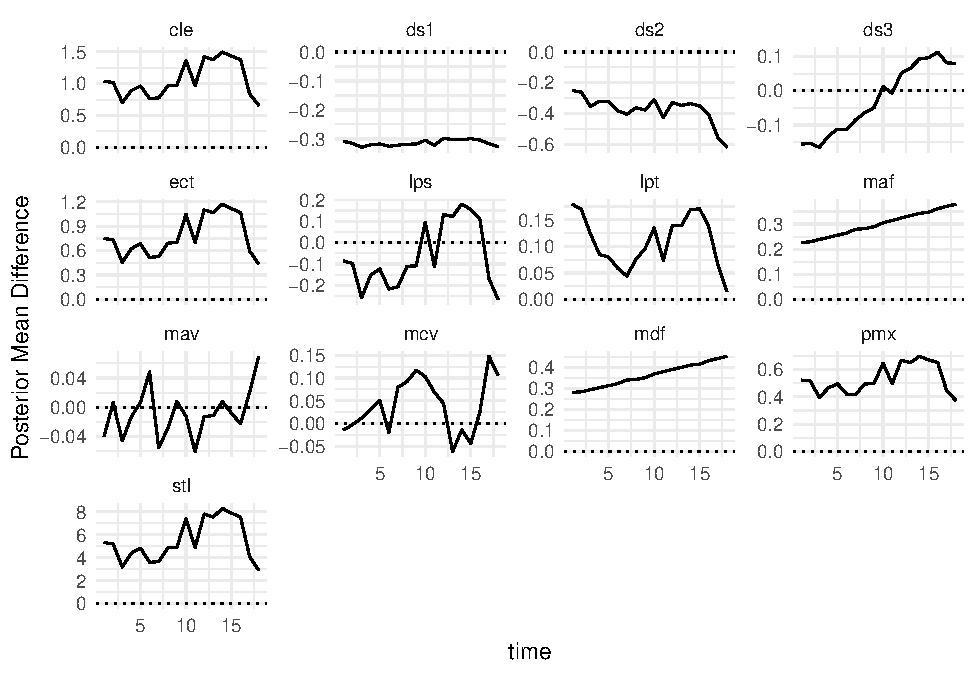
\includegraphics{paper_files/figure-latex/mu-diff-plot-1} 

}

\caption{Posterior mean difference between males and females, in UNITS?. Values above 0 indicate larger male means}\label{fig:mu-diff-plot}
\end{figure}

\begin{figure}

{\centering 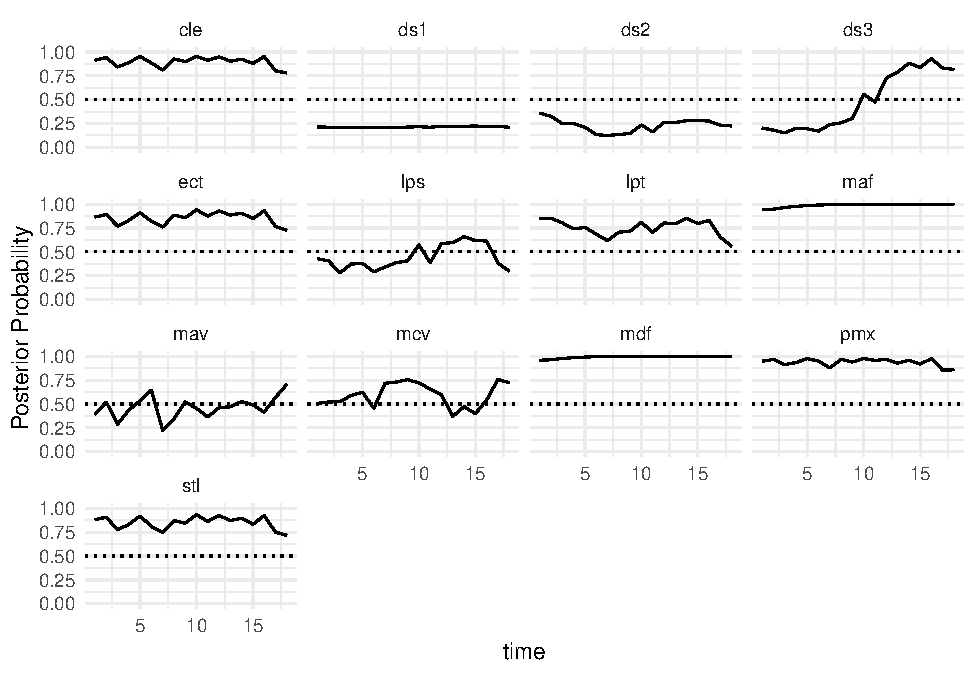
\includegraphics{paper_files/figure-latex/prob0-plot-1} 

}

\caption{Posterior probabilities that the male posterior mean is larger than the female posterior mean}\label{fig:prob0-plot}
\end{figure}

\begin{figure}

{\centering 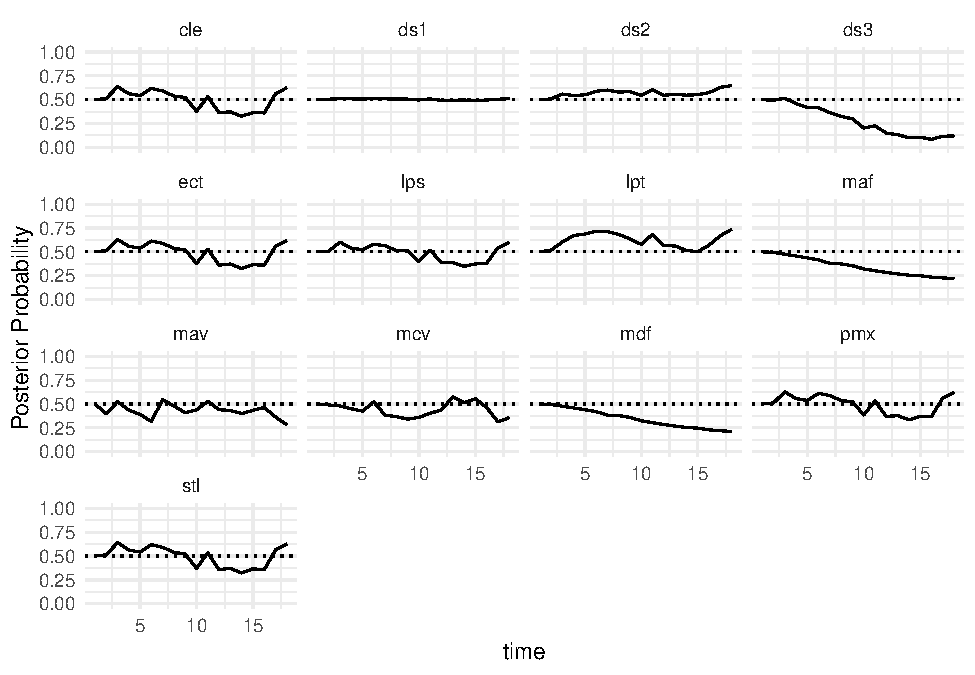
\includegraphics{paper_files/figure-latex/AUC-plot-1} 

}

\caption{The Posterior Probability that male-female differences in subsequent samples are different from male-female differenceds in the initial sample. Values near 0.5 indicate little difference between the distributions. Values closer to 0 indicate that the difference in means has shifted towards larger means in females. Values closer to 1 indicate that the difference in means has shifted toward larger means in males.}\label{fig:AUC-plot}
\end{figure}

\hypertarget{sec:conclusions}{%
\section{Discussion, Future work and
conclusions}\label{sec:conclusions}}

We predicted that release from predators would result in niche expansion
and increased sexual dimorphism, based on several studies of modern
stickleback. For example, in lakes where sculpin competitors are absent
and stickleback (Roesti et al.~2023) See Spoljaric and Reimchen 2008,
page 512 right column for references and discussion of differences
between benthic males and limnetic females. Male stickleback are benthic
and littoral (Wootton 1976)\ldots. Reimchen papers in general good for
this section.

\hypertarget{acknowledgements}{%
\section*{Acknowledgements}\label{acknowledgements}}
\addcontentsline{toc}{section}{Acknowledgements}

We thank O. Abughoush, S. Blain, A. Chaudhary, M. Islam, F. Joaquin, C.
Lawson-Weinert, R. Sullivan, J. Tien, M.P. Travis, and W. Shim for help
with data collection. We thank D. Schluter and S. Blain for loaning
specimens and sharing data. We thank K. Swagel and C. McMahan of the
Field Museum for assistance with specimen x-rays. This research was
supported by NSF grants BSR-8111013, EAR-9870337, and DEB-0322818, the
Center for Field Research (Earthwatch), and the National Geographic
Society (2869-84) to MAB. It was also supported by NSF grants
DEB-1456462 and EAR-2145830 to YES. And NSF DMS-2015374 (GJM)

\hypertarget{supplementary-material}{%
\section*{Supplementary Material}\label{supplementary-material}}
\addcontentsline{toc}{section}{Supplementary Material}

All code for reproducing the analyses in this paper is publicly
available at \url{https://github.com/Akhil-Ghosh/SticklebackProject}

DIC results here.

\hypertarget{figures}{%
\subsection{Figures}\label{figures}}

\begin{figure}

{\centering 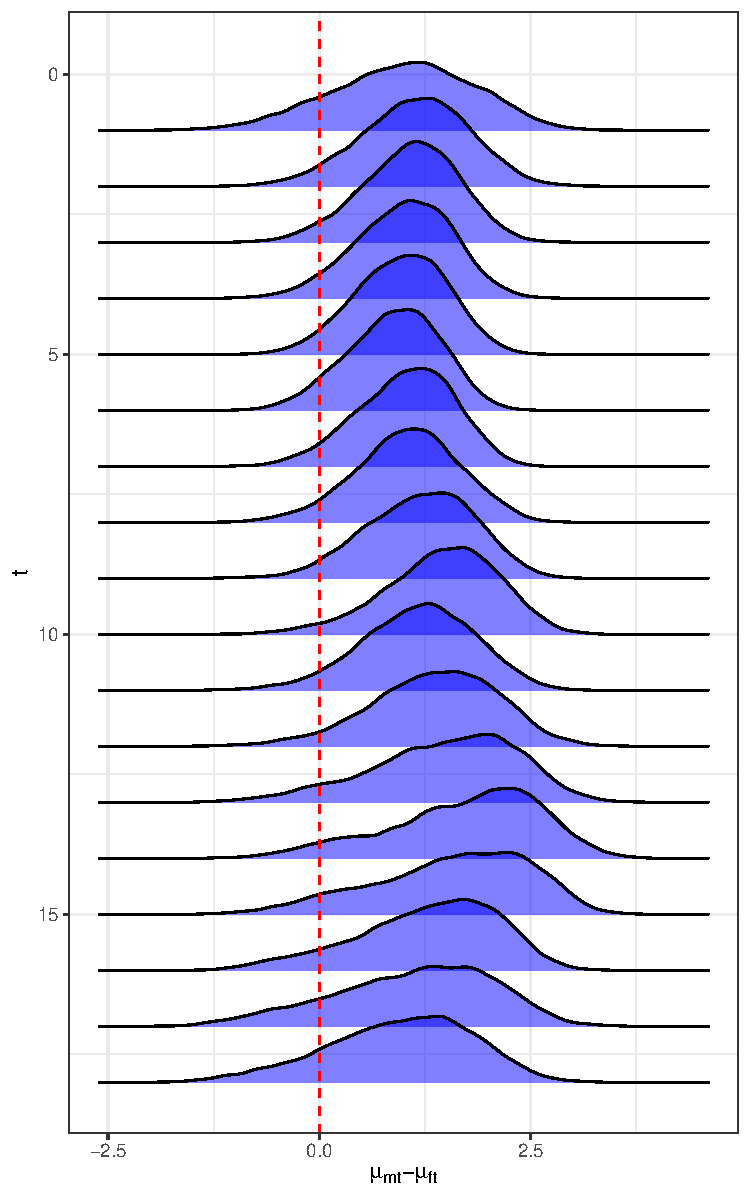
\includegraphics[width=0.9\linewidth]{../Figures/cle/mu_diff} 

}

\caption{cle}\label{fig:unnamed-chunk-7}
\end{figure}
\begin{figure}

{\centering 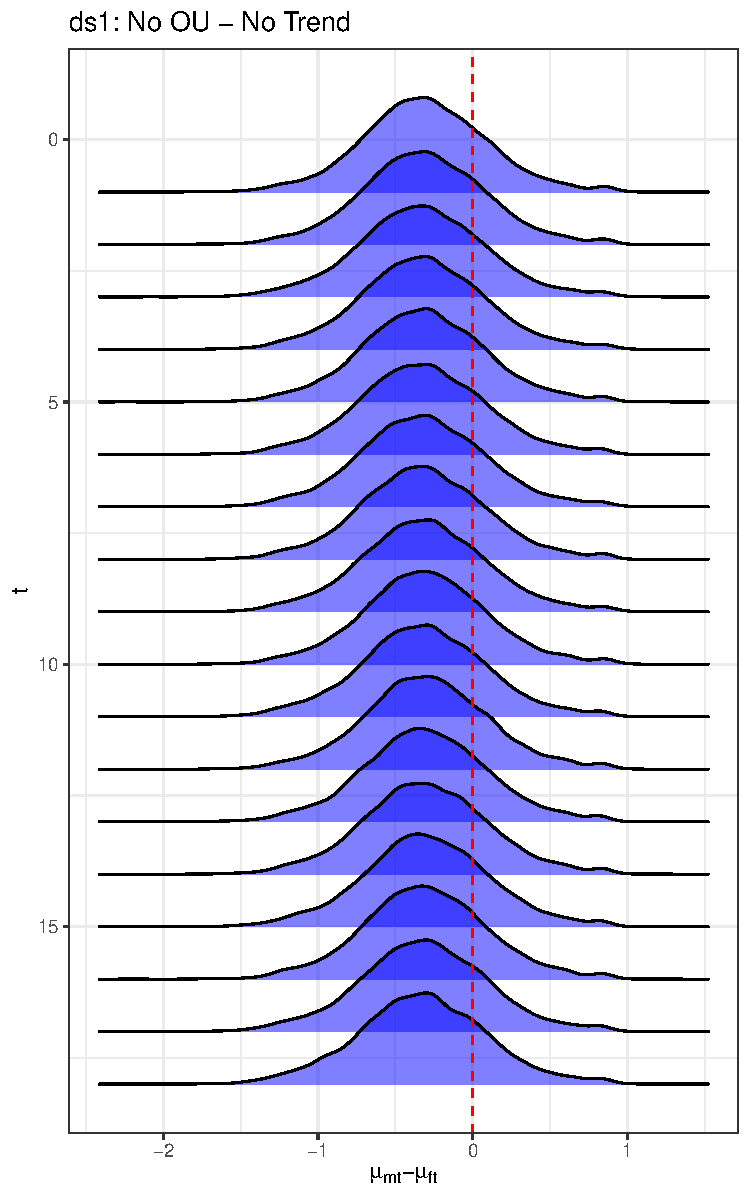
\includegraphics[width=0.9\linewidth]{../Figures/ds1/mu_diff} 

}

\caption{ds1}\label{fig:unnamed-chunk-8}
\end{figure}
\begin{figure}

{\centering 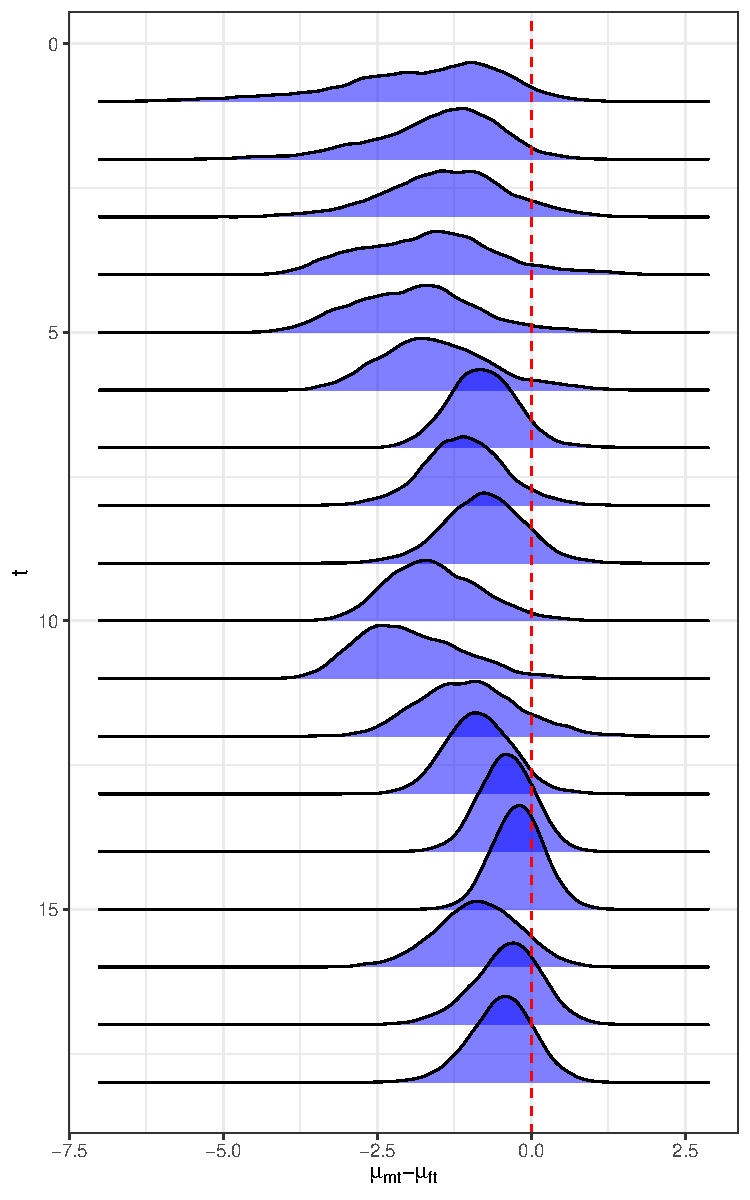
\includegraphics[width=0.9\linewidth]{../Figures/ds2/mu_diff} 

}

\caption{ds2}\label{fig:unnamed-chunk-9}
\end{figure}
\begin{figure}

{\centering 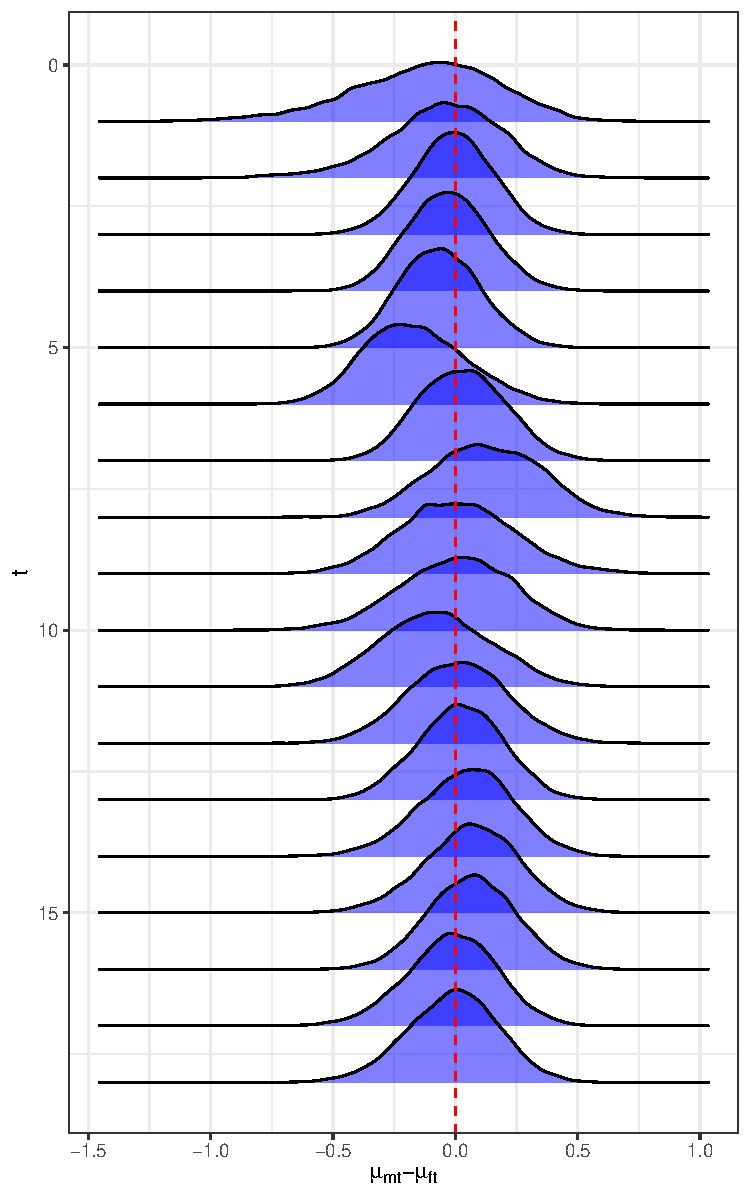
\includegraphics[width=0.9\linewidth]{../Figures/ds3/mu_diff} 

}

\caption{ds3}\label{fig:unnamed-chunk-10}
\end{figure}
\begin{figure}

{\centering 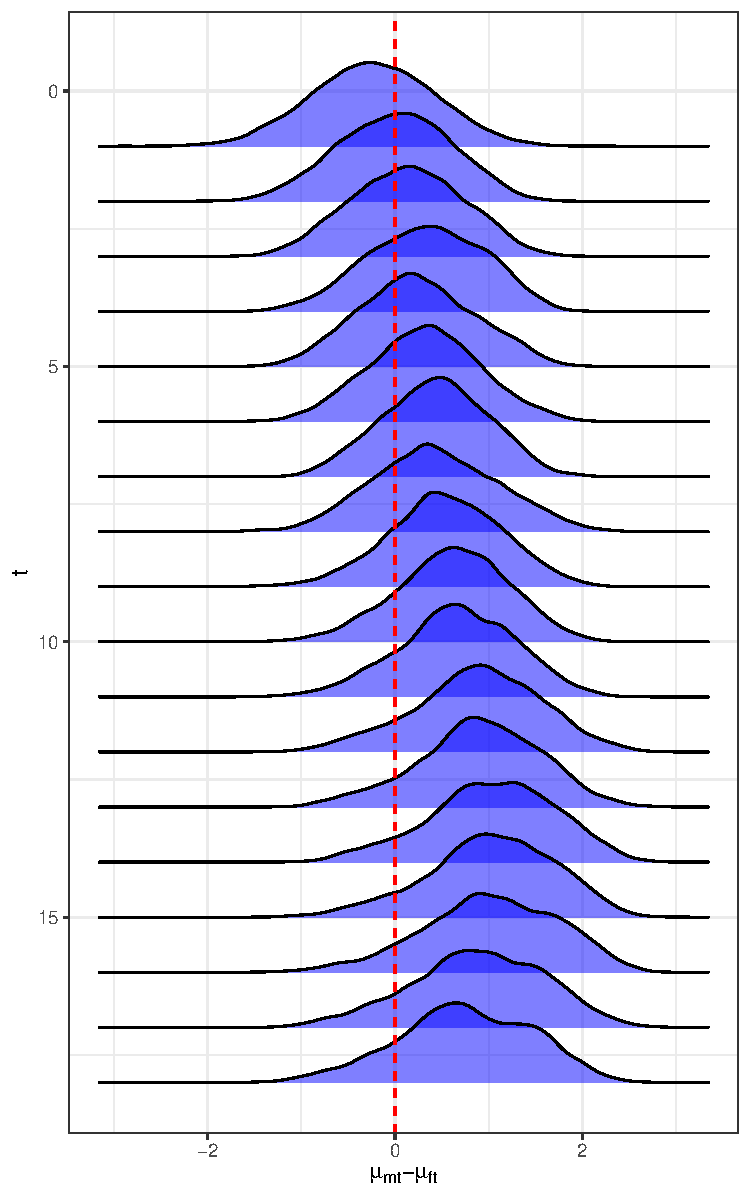
\includegraphics[width=0.9\linewidth]{../Figures/ect/mu_diff} 

}

\caption{ect}\label{fig:unnamed-chunk-11}
\end{figure}
\begin{figure}

{\centering 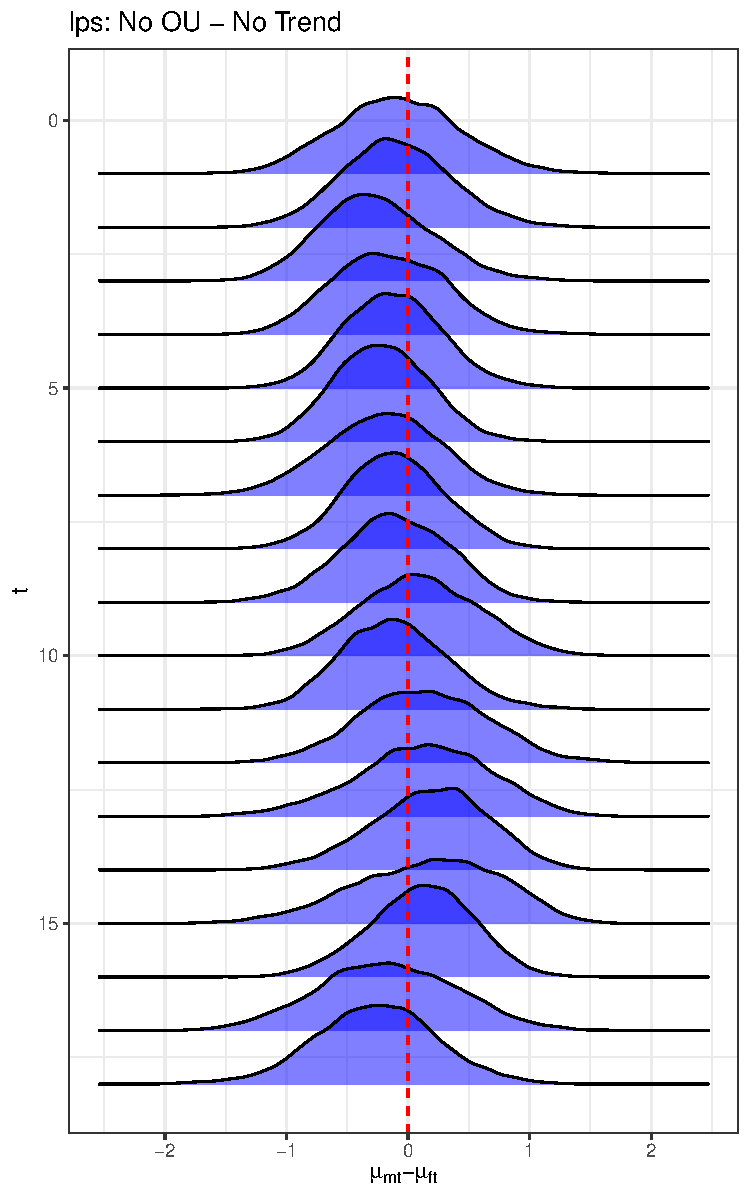
\includegraphics[width=0.9\linewidth]{../Figures/lps/mu_diff} 

}

\caption{lps}\label{fig:unnamed-chunk-12}
\end{figure}
\begin{figure}

{\centering 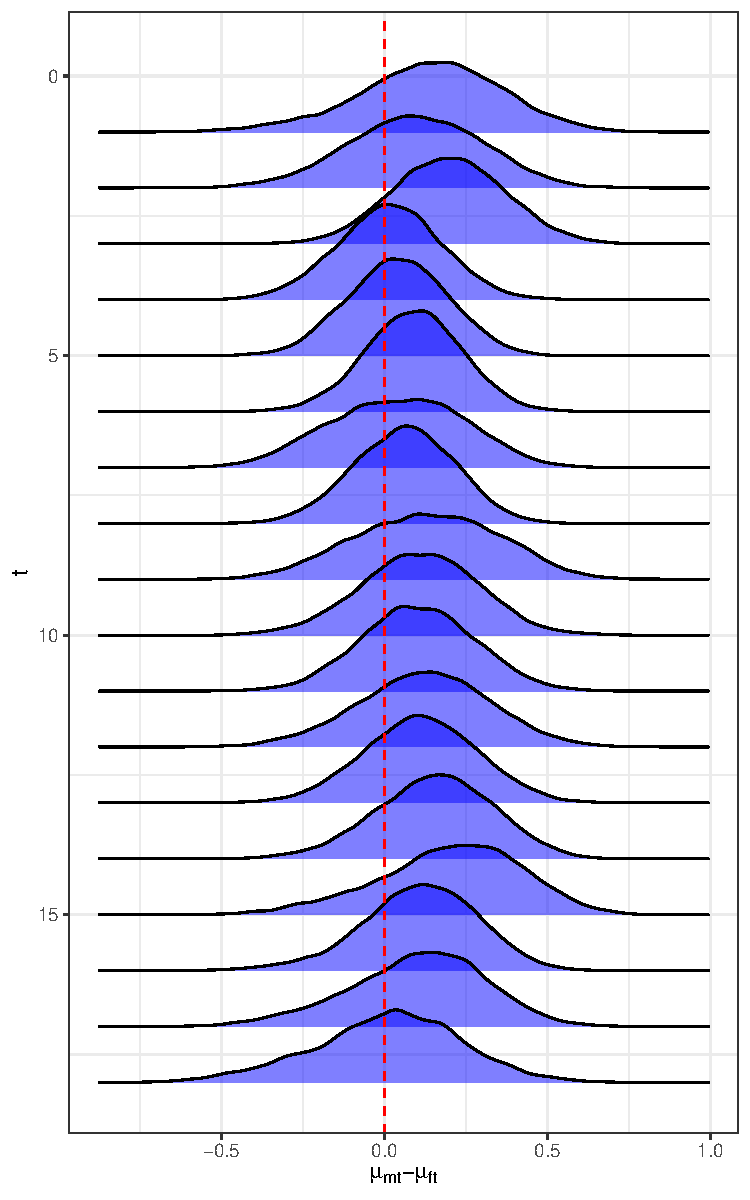
\includegraphics[width=0.9\linewidth]{../Figures/lpt/mu_diff} 

}

\caption{lpt}\label{fig:unnamed-chunk-13}
\end{figure}
\begin{figure}

{\centering 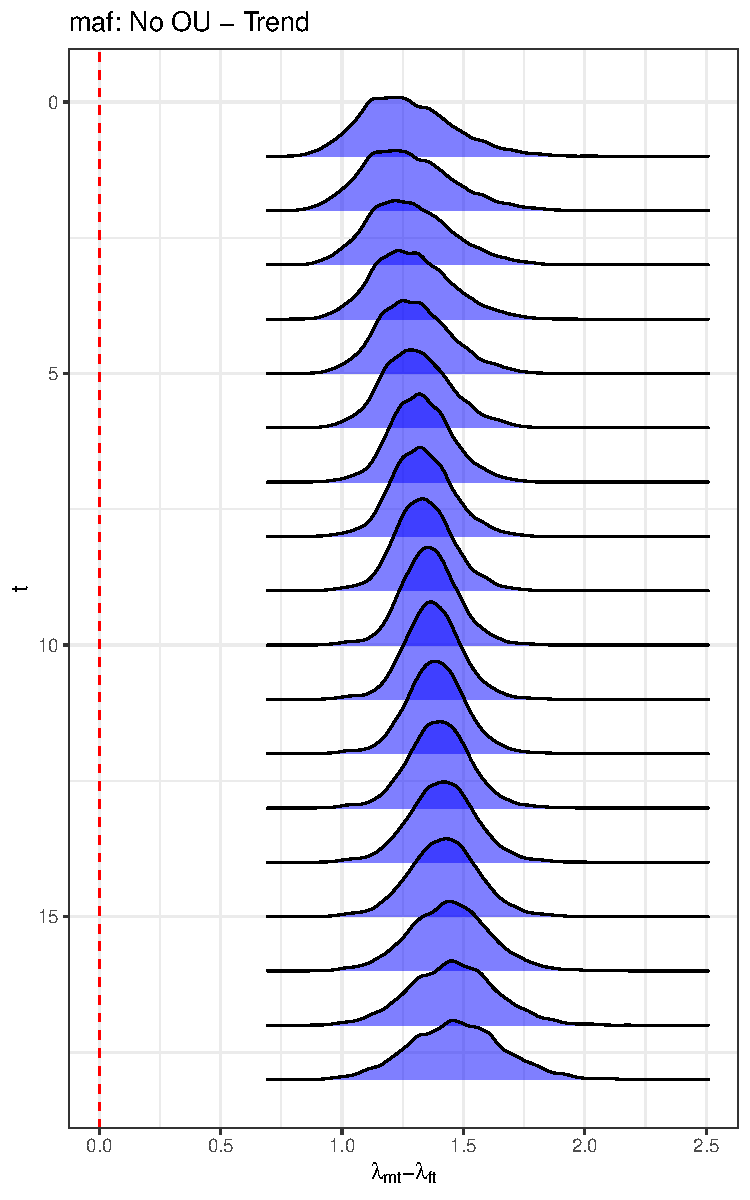
\includegraphics[width=0.9\linewidth]{../Figures/maf/lambda_diff} 

}

\caption{maf}\label{fig:unnamed-chunk-14}
\end{figure}
\begin{figure}

{\centering 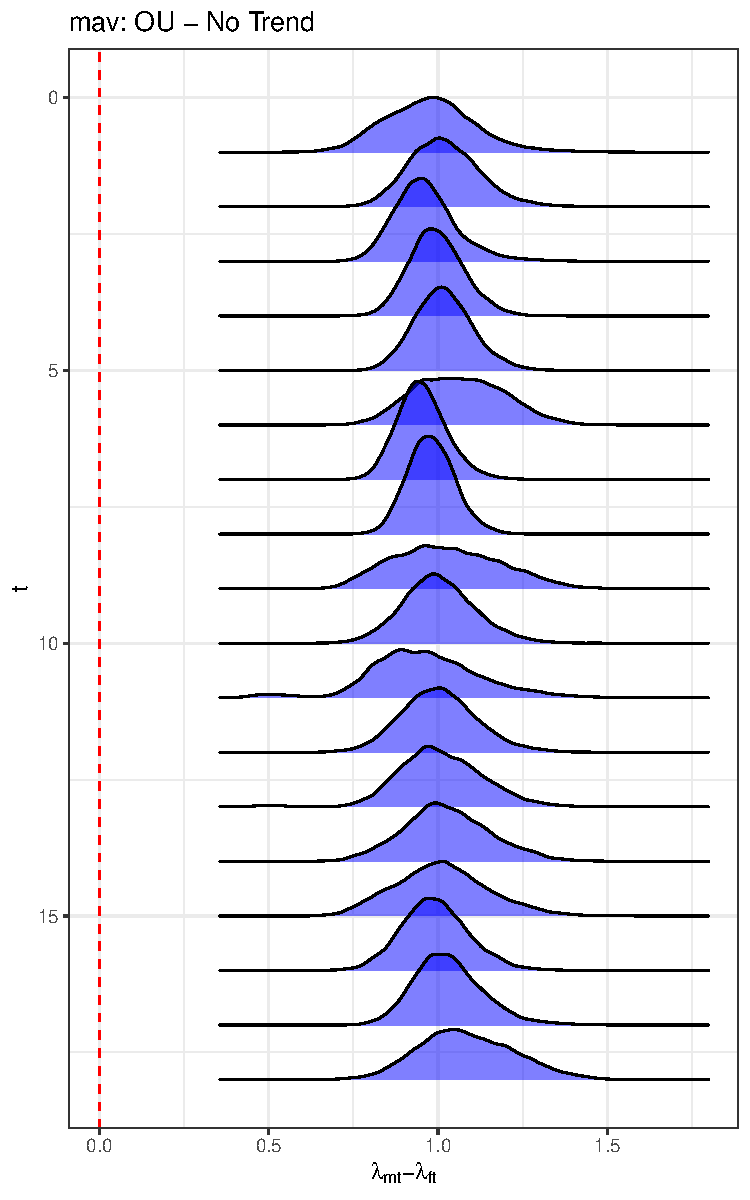
\includegraphics[width=0.9\linewidth]{../Figures/mav/lambda_diff} 

}

\caption{mav}\label{fig:unnamed-chunk-15}
\end{figure}
\begin{figure}

{\centering 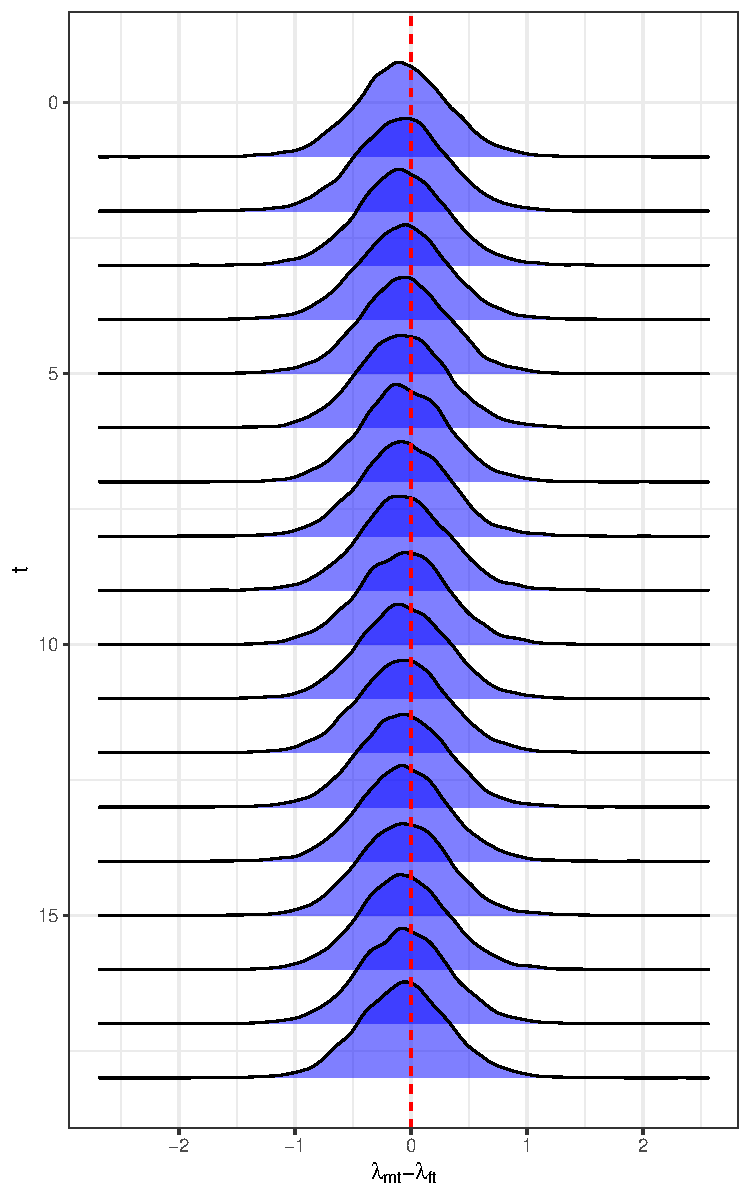
\includegraphics[width=0.9\linewidth]{../Figures/mcv/lambda_diff} 

}

\caption{mcv}\label{fig:unnamed-chunk-16}
\end{figure}
\begin{figure}

{\centering 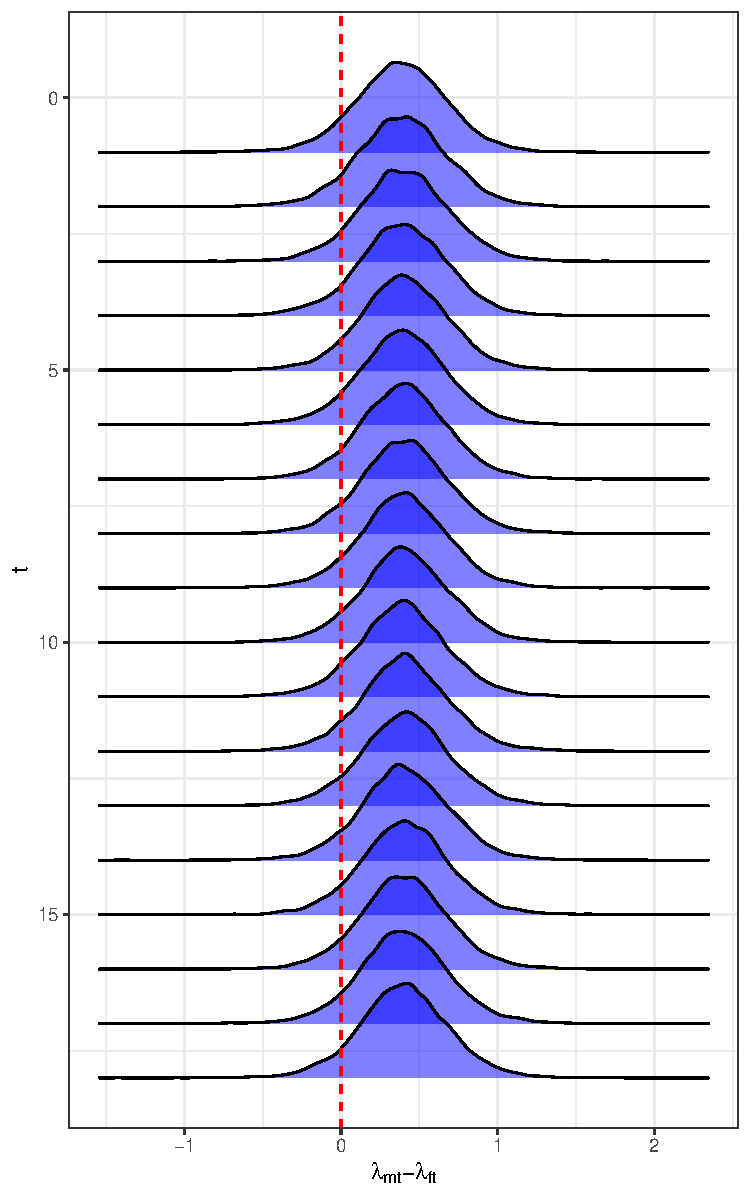
\includegraphics[width=0.9\linewidth]{../Figures/mdf/lambda_diff} 

}

\caption{mdf}\label{fig:unnamed-chunk-17}
\end{figure}
\begin{figure}

{\centering 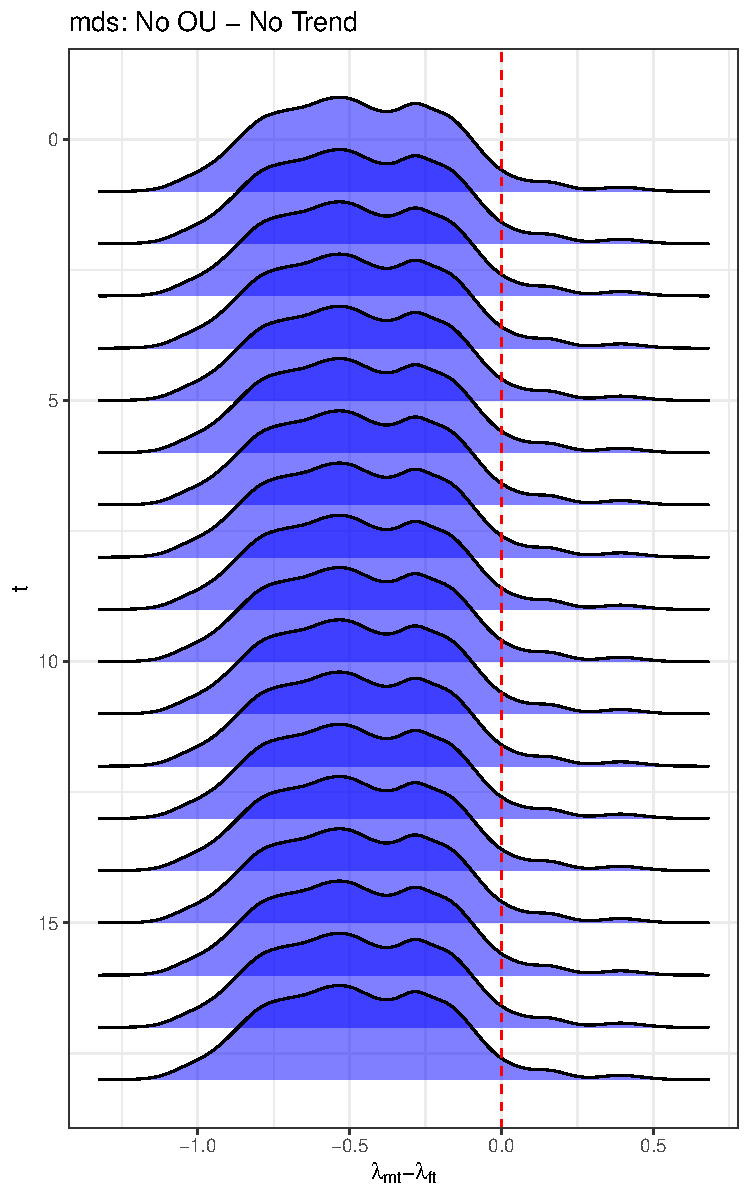
\includegraphics[width=0.9\linewidth]{../Figures/mds/lambda_diff} 

}

\caption{mds}\label{fig:unnamed-chunk-18}
\end{figure}
\begin{figure}

{\centering 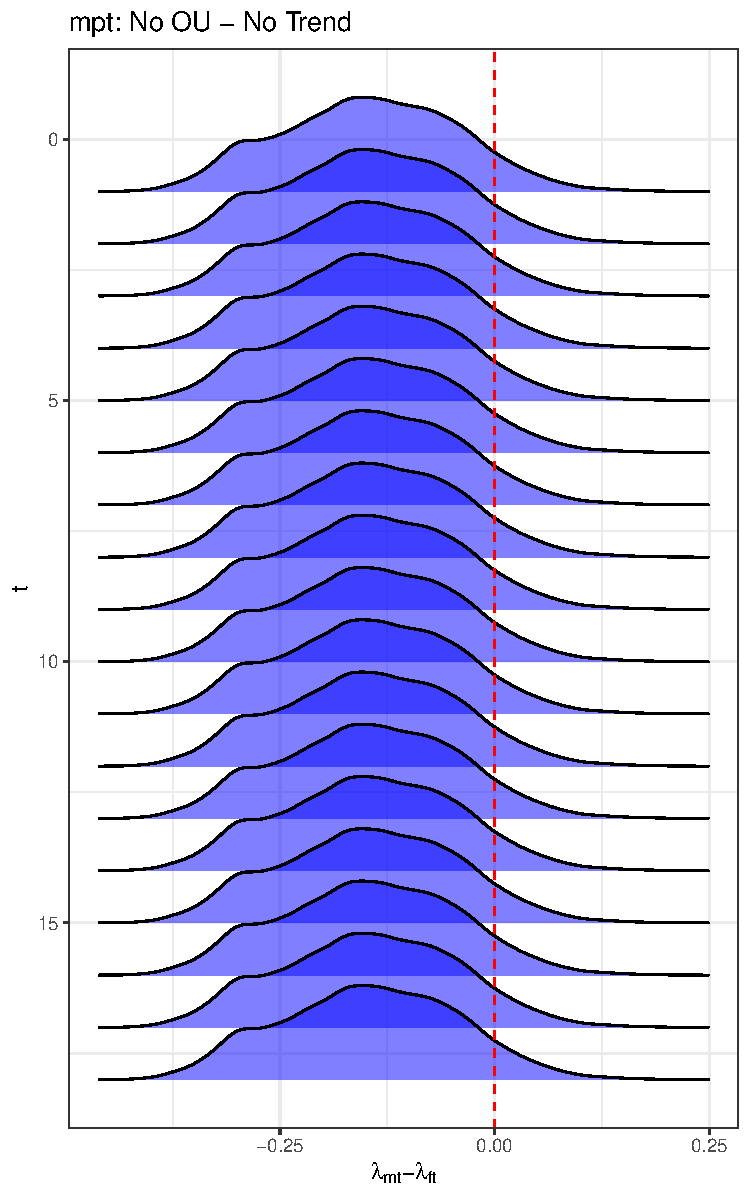
\includegraphics[width=0.9\linewidth]{../Figures/mpt/lambda_diff} 

}

\caption{mpt}\label{fig:unnamed-chunk-19}
\end{figure}
\begin{figure}

{\centering 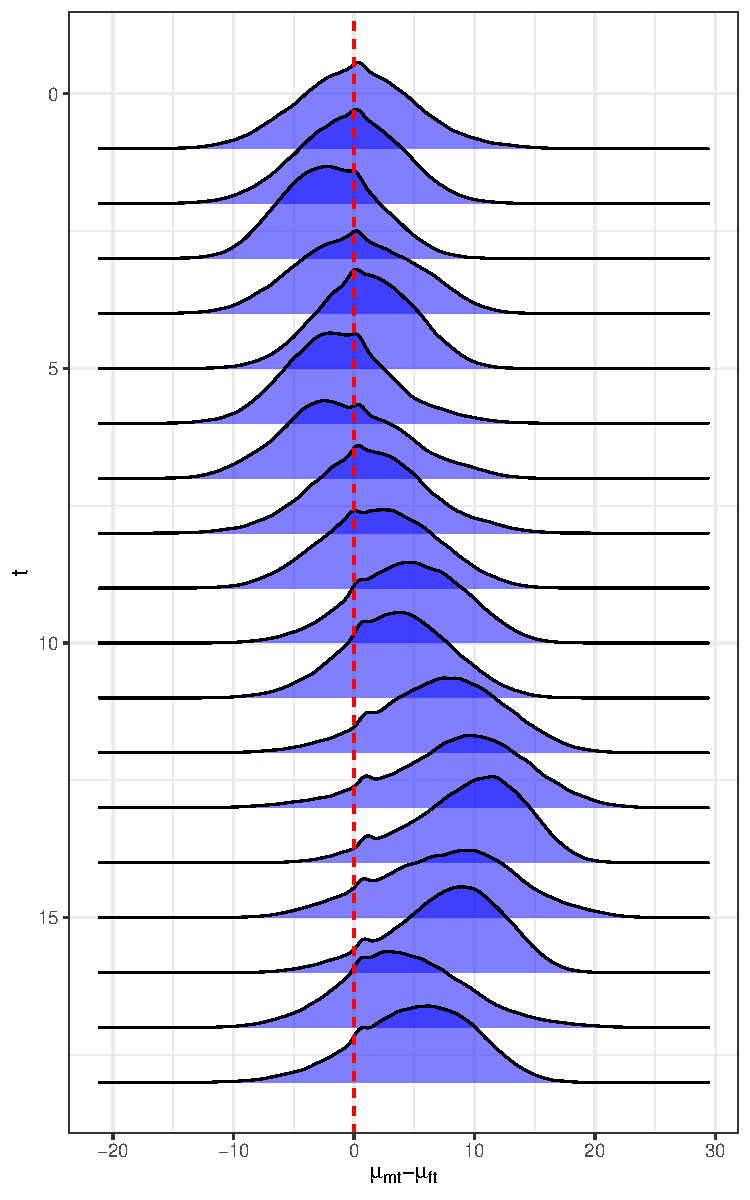
\includegraphics[width=0.9\linewidth]{../Figures/pmx/mu_diff} 

}

\caption{pmx}\label{fig:unnamed-chunk-20}
\end{figure}

\begin{figure}

{\centering 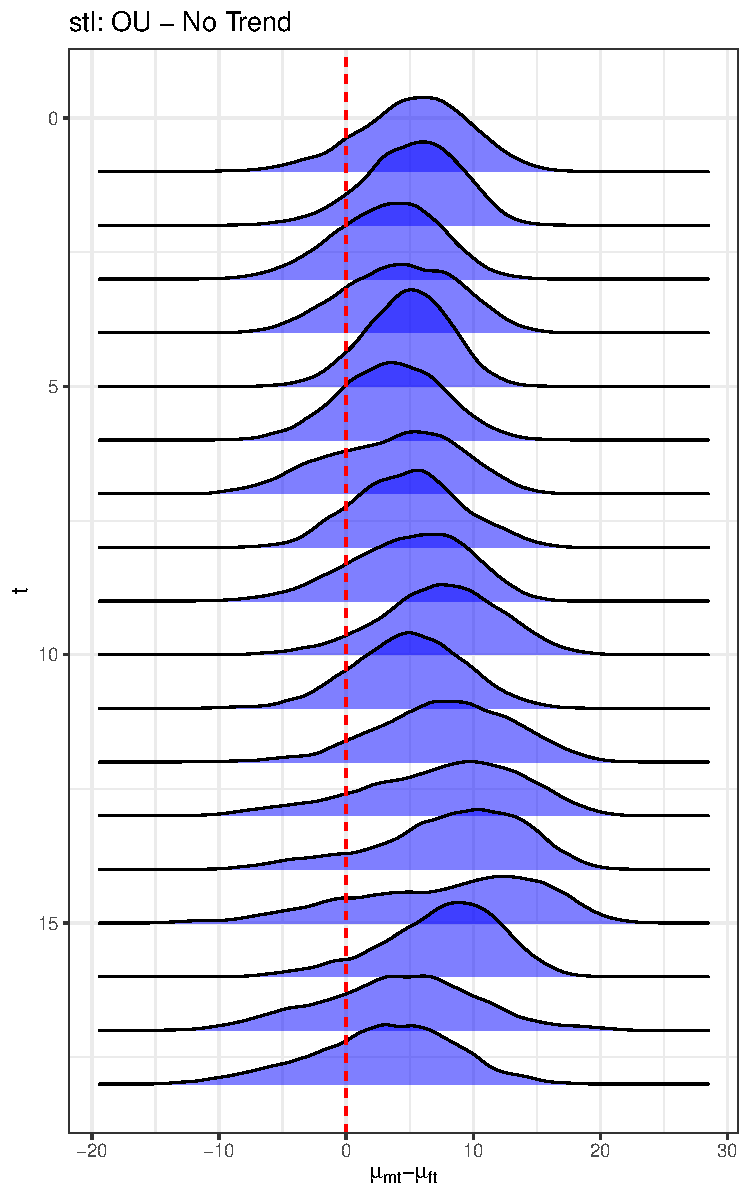
\includegraphics[width=0.9\linewidth]{../Figures/stl/mu_diff} 

}

\caption{stl}\label{fig:unnamed-chunk-21}
\end{figure}

\hypertarget{references}{%
\section*{References}\label{references}}
\addcontentsline{toc}{section}{References}

\hypertarget{refs}{}
\begin{CSLReferences}{1}{0}
\leavevmode\vadjust pre{\hypertarget{ref-Aguirreetal2014}{}}%
Aguirre, W E, K Walker, and S Gideon. 2014. {``Tinkering with the Axial
Skeleton: Vertebral Number Variation in Ecologically Divergent
Threespine Stickleback Populations.''} \emph{Biological Journal of the
Linnean Society} 113 (1): 204--19.

\leavevmode\vadjust pre{\hypertarget{ref-Baumgartneretal1988}{}}%
Baumgartner, J V, M A Bell, and P H Weinberg. 1988. {``Body Form
Differences Between the Enos Lake Species Pair of Threespine
Sticklebacks (Gasterosteus Aculeatus Complex).''} \emph{Canadian Journal
of Zoology} 66 (2): 467--74.

\leavevmode\vadjust pre{\hypertarget{ref-Bell2009}{}}%
Bell, M A. 2009. {``Implications of a Fossil Stickleback Assemblage for
Darwinian Gradualism.''} \emph{Journal of Fish Biology} 75 (8):
1977--99.

\leavevmode\vadjust pre{\hypertarget{ref-Belletal1985}{}}%
Bell, M A, J V Baumgartner, and E C Oslon. 1985. {``Patterns of Temporal
Change in Single Morphological Characters of a Miocene Stickleback
Fish.''} \emph{Paleobiology} 11: 258--71.

\leavevmode\vadjust pre{\hypertarget{ref-Belletal1993}{}}%
Bell, M A, G Orti, J A Walker, and J P Koenings. 1993. {``Evolution of
Pelvic Reduction in Threespine Sticklebacks: A Test of Competing
Hypotheses.''} \emph{Evolution} 47: 906--14.

\leavevmode\vadjust pre{\hypertarget{ref-Belletal2006}{}}%
Bell, M A, M P Travis, and D M Blouw. 2006. {``Inferring Natural
Selection in a Fossil Threespine Stickleback.''} \emph{Paleobiology} 32
(4): 562--77.

\leavevmode\vadjust pre{\hypertarget{ref-Blain2022}{}}%
Blain, S A. 2022. \emph{Evolutionary Outcomes of Interactions Among
Phenotypes in Post-Glacial Lakes}. University of British Columbia,
Canada.

\leavevmode\vadjust pre{\hypertarget{ref-Bolnick2011}{}}%
Bolnick, D I. 2011. {``Sympatric Speciation in Threespine Stickleback:
Why Not?''} \emph{International Journal of Ecology} 2011: 1--15.

\leavevmode\vadjust pre{\hypertarget{ref-BolnickandDoebeli2003}{}}%
Bolnick, D I, and M Doebeli. 2003. {``Sexual Dimorphism and Adaptive
Speciation: Two Sides of the Same Ecological Coin.''} \emph{Evolution}
57 (11): 2433--49.

\leavevmode\vadjust pre{\hypertarget{ref-BolnickandLau2008}{}}%
Bolnick, D I, and O L Lau. 2008. {``Predictable Patterns of Disruptive
Selection in Stickleback in Postglacial Lakes.''} \emph{The American
Naturalist} 172 (1): 1--11.

\leavevmode\vadjust pre{\hypertarget{ref-Bowne1994}{}}%
Bowne, P S. 1994. {``Systematics and Morphology of the
Gasterosteiformes.''} In \emph{The Evolutionary Biology of the
Threespine Stickleback}, edited by M A Bell and S A Foster. Oxford, UK:
Oxford University Press.

\leavevmode\vadjust pre{\hypertarget{ref-Butleretal2007}{}}%
Butler, Sawyer, M A, and J B Losos. 2007. {``Sexual Dimorphism and
Adaptive Radiation in Anolis Lizards.''} \emph{Nature} 447 (7141):
202--5.

\leavevmode\vadjust pre{\hypertarget{ref-MICE}{}}%
Buuren, Stef van, and Karin Groothuis-Oudshoorn. 2011. {``Mice:
Multivariate Imputation by Chained Equations in r.''} \emph{Journal of
Statistical Software} 45 (3): 1--67.
\url{https://doi.org/10.18637/jss.v045.i03}.

\leavevmode\vadjust pre{\hypertarget{ref-Cerasonietal2024}{}}%
Cerasoni, J N, M A Bell, and Y E Stuart. 2024. {``Geology,
Microstratigraphy, and Paleontology of Truckee Formation Lacustrine
Diatomite Deposits Near Hazen, Nevada, USA, with Emphasis on Fossil
Stickleback Fish.''} \emph{PaleoBios} 41: 1--15.

\leavevmode\vadjust pre{\hypertarget{ref-Cooperetal2011}{}}%
Cooper, I A, R T Gilman, and J W Boughman. 2011. {``Sexual Dimorphism
and Speciation on Two Ecological Coins: Patterns from Nature and
Theoretical Predictions.''} \emph{Evolution} 65 (9): 2553--71.

\leavevmode\vadjust pre{\hypertarget{ref-Cornault2022}{}}%
Cornuault, J. 2022. {``Bayesian Analyses of Comparative Data with the
Ornstein--Uhlenbeck Model: Potential Pitfalls.''} \emph{Systematic
Biology} 71 (6): 1524--40. \url{https://doi.org/10.1093/sysbio/syac036}.

\leavevmode\vadjust pre{\hypertarget{ref-DeLisleetal2018}{}}%
De Lisle, S P, S Paiva, and L Rowe. 2018. {``Habitat Partitioning During
Character Displacement Between the Sexes.''} \emph{Biology Letters} 14:
20180124.

\leavevmode\vadjust pre{\hypertarget{ref-DeLisleandRowe2015}{}}%
De Lisle, S P, and L Rowe. 2015. {``Ecological Character Displacement
Between the Sexes.''} \emph{The American Naturalist} 186: 693--707.

\leavevmode\vadjust pre{\hypertarget{ref-DeLisleandRowe2017}{}}%
---------. 2017. {``Disruptive Natural Selection Predicts Divergence
Between the Sexes During Adaptive Radiation.''} \emph{Ecology and
Evolution} 7: 3590--3601.

\leavevmode\vadjust pre{\hypertarget{ref-Godfreyetal1993}{}}%
Godfrey, L R, S K Lyon, and M R Sutherland. 1993. {``Sexual Dimorphism
in Large-Bodied Primates: The Case of the Subfossil Lemurs.''}
\emph{American Journal of Physical Anthropology} 90: 315--34.

\leavevmode\vadjust pre{\hypertarget{ref-Hendryetal2009}{}}%
Hendry, A P, D I Bolnick, D Berner, and C L Peichel. 2009. {``Along the
Speciation Continuum in Sticklebacks.''} \emph{Journal of Fish Biology}
75 (8): 2000--2036.

\leavevmode\vadjust pre{\hypertarget{ref-Herrmannetal2021}{}}%
Herrmann, N C, J T Stroud, and J B Losos. 2021. {``The Evolution of
'Ecological Release' into the 21st Century.''} \emph{Trends in Ecology
and Evolution} 36 (3): 206--15.

\leavevmode\vadjust pre{\hypertarget{ref-HoneandMallon2017}{}}%
Hone, D W E, and J C Mallon. 2017. {``Protracted Growth Impedes the
Detection of Sexual Dimorphism in Non-Avian Dinosaurs.''}
\emph{Palaeontology} 60 (4): 535--45.

\leavevmode\vadjust pre{\hypertarget{ref-Huntetal2008}{}}%
Hunt, G, M A Bell, and M P Travis. 2008. {``Evolution Toward a New
Adaptive Optimum: Phenotypic Evolution in a Fossil Stickleback
Lineage.''} \emph{Evolution} 62 (3): 700--710.

\leavevmode\vadjust pre{\hypertarget{ref-KoscinskiandPietraszewski2004}{}}%
Koscinski, K, and S Pietraszewski. 2004. {``Methods to Estimate Sexual
Dimorphism from Unsexed Samples: A Test with Computer Generated
Samples.''} \emph{Przeglad Antropologiczny - Anthropological Review} 67:
33--55.

\leavevmode\vadjust pre{\hypertarget{ref-little2002statistical}{}}%
Little, R. J. A., and D. B. Rubin. 2002. \emph{Statistical Analysis with
Missing Data}. Wiley Series in Probability and Mathematical Statistics.
Probability and Mathematical Statistics. Wiley.
\url{http://books.google.com/books?id=aYPwAAAAMAAJ}.

\leavevmode\vadjust pre{\hypertarget{ref-Mallon2017}{}}%
Mallon, J C. 2017. {``Recognizing Sexual Dimorphism in the Fossil
Record: Lessons from Nonavian Dinosaurs.''} \emph{Paleobiology} 43 (3):
495--507.

\leavevmode\vadjust pre{\hypertarget{ref-ParentandCrespi2009}{}}%
Parent, C E, and B J Crespi. 2009. {``Ecological Opportunity in Adaptive
Radiation of Galapagos Endemic Land Snails.''} \emph{The American
Naturalist} 174: 898--905.

\leavevmode\vadjust pre{\hypertarget{ref-PfennigandPfennig2012}{}}%
Pfennig, D W, and K S Pfennig. 2012. \emph{\href{}{Evolution's Wedge:
Competition and the Origins of Diversity}}. University of California
Press, Berkeley, USA.

\leavevmode\vadjust pre{\hypertarget{ref-Reimchen1994}{}}%
Reimchen, T E. 1994. {``Predators and Morphological Evolution in
Threespine Stickleback.''} In \emph{The Evolutionary Biology of the
Threespine Stickleback}, edited by M A Bell and S A Foster. Oxford, UK:
Oxford University Press.

\leavevmode\vadjust pre{\hypertarget{ref-ReimchenandNosil2004}{}}%
Reimchen, T E, and P Nosil. 2004. {``Variable Predation Regimes Predict
the Evolution of Sexual Dimorphism in a Population of Threespine
Stickleback.''} \emph{Evolution} 58 (6): 1274--81.

\leavevmode\vadjust pre{\hypertarget{ref-Roestietal2023}{}}%
Roesti, M, J S Groh, S A Blain, M Huss, P Rassias, D I Bolnick, Y E
Stuart, C L Peichel, and D Schluter. 2023. {``Species Divergence Under
Competition and Shared Predation.''} \emph{Ecology Letters} 26: 111--23.

\leavevmode\vadjust pre{\hypertarget{ref-Saittaetal2020}{}}%
Saitta, T, M T Stockdale, N R Longrich, V Bonhomme, M J Benton, I C
Cuthill, and P J Makovicky. 2020. {``An Effect Size Statistical
Framework for Investigating Sexual Dimorphism in Non-Avian Dinosaurs and
Other Extinct Taxa.''} \emph{Biological Journal of the Linnean Society}
131 (2): 231--73. \url{https://doi.org/10.1093/biolinnean/blaa105}.

\leavevmode\vadjust pre{\hypertarget{ref-Schindelinetal2012}{}}%
Schindelin, J, I Arganda-Carreras, E Frise, V Kaynig, M Longair, T
Pietzsch, S Preibisch, C Rueden, S Saalfeld, and B Schmid. 2012.
{``Fiji: An Open-Source Platform for Biological-Image Analysis.''}
\emph{Nature Methods} 9: 976--682.

\leavevmode\vadjust pre{\hypertarget{ref-SchluterandMcPhail1992}{}}%
Schluter, D, and J D McPhail. 1992. {``Ecological Character Displacement
and Speciation in Sticklebacks.''} \emph{The American Naturalist} 140
(1): 85--108.

\leavevmode\vadjust pre{\hypertarget{ref-Schoener1968}{}}%
Schoener, T W. 1968. {``The Anolis Lizards of Bimini: Resource
Partitioning in a Complex Fauna.''} \emph{Ecology} 29: 704--26.

\leavevmode\vadjust pre{\hypertarget{ref-Shine1989}{}}%
Shine, R. 1989. {``Ecological Causes for the Evolution of Sexual
Dimorphism: A Review of the Evidence.''} \emph{The Quarterly Review of
Biology} 64 (4): 419--61.

\leavevmode\vadjust pre{\hypertarget{ref-Siddiquietal2024}{}}%
Siddiqui, R, S Swank, A Ozark, F Joaquin, M P Travis, C D McMahan, M A
Bell, and Y E Stuart. 2024. {``Inferring the Evolution of Reproductive
Isolation in a Lineage of Fossil Threespine Stickleback, Gasterosteus
Doryssus.''} \emph{Proceedings of the Royal Society B} 291: 20240337.

\leavevmode\vadjust pre{\hypertarget{ref-Stuartetal2021}{}}%
Stuart, Y E, J W Sherwin, A Kamath, and T Veen. 2021. {``Male and Female
Anolis Carolinensis Maintain Their Dimorphism Despite the Presence of
Novel Interspecific Competition.''} \emph{Evolution} 75 (11): 2708--16.

\leavevmode\vadjust pre{\hypertarget{ref-Stuartetal2020}{}}%
Stuart, Y E, M P Travis, and M A Bell. 2020. {``Inferred Genetic
Architecture Underlying Evolution in a Fossil Stickleback Lineage.''}
\emph{Nature Ecology and Evolution} 4 (11): 1549--57.

\leavevmode\vadjust pre{\hypertarget{ref-Stuartetal2017}{}}%
Stuart, Y E, T Veen, J N Weber, D Hanson, M Ravinet, B K Lohman, C J
Thompson, et al. 2017. {``Contrasting Effects of Environment and
Genetics Generate a Continuum of Parallel Evolution.''} \emph{Nature
Ecology and Evolution} 1 (6): 158.

\leavevmode\vadjust pre{\hypertarget{ref-R2022language}{}}%
Team, R Core. 2022. \emph{R: A Language and Environment for Statistical
Computing}. Vienna, Austria: R Foundation for Statistical Computing.
\url{https://www.R-project.org/}.

\leavevmode\vadjust pre{\hypertarget{ref-OUProcess}{}}%
Uhlenbeck, G E, and L S Ornstein. 1930. {``On the Theory of the Brownian
Motion.''} \emph{Phys. Rev.} 36 (September): 823--41.
\url{https://doi.org/10.1103/PhysRev.36.823}.

\leavevmode\vadjust pre{\hypertarget{ref-VamosiandSchluter2004}{}}%
Vamosi, S M, and D Schluter. 2004. {``Character Shifts in the Defensive
Armor of Sympatric Sticklebacks.''} \emph{Evolution} 58: 376--85.

\leavevmode\vadjust pre{\hypertarget{ref-Vojeetal2022}{}}%
Voje, K L, M A Bell, and Y E Stuart. 2022. {``Evolution of Static
Allometry and Constraint on Evolutionary Allometry in a Fossil
Stickleback.''} \emph{Journal of Evolutionary Biology} 35 (3): 423--38.

\leavevmode\vadjust pre{\hypertarget{ref-ZhouReiter2010}{}}%
Zhou, X, and J Reiter. 2010. {``A Note on Bayesian Inference After
Multiple Imputation.''} \emph{The American Statistician} 64 (2):
159--63.

\end{CSLReferences}

\end{document}
